\chapter{Influence of combined temperature and food availability on Peruvian anchovy (\textit{Engraulis ringens}) early life stages in the northern Humboldt Current system:\\A modelling approach}\label{Chap3}

\clearpage
This chapter is based on the following published scientific paper \citep{FlorLett2023} \textbf{\textit{Influence of combined temperature and food availability on Peruvian anchovy (\gls{ringens}) early life stages in the northern Humboldt Current system: A modelling approach.}}\\

Available at: \href{https://www.sciencedirect.com/science/article/abs/pii/S0079661123000770}{Progress in Oceanography}.

\clearpage
\section*{Abstract}

In the \acrfull{nhcs}, the Peruvian anchovy (\textit{\gls{ringens}}) constitutes the bulk of landings and has a significant socioeconomic contribution. Understanding the impact of environment on the early-life stages of anchovy and further population dynamics remains challenging. Climate variability at a variety of scales modulates currents velocity, temperature and food availability, impacting early-life stages drift, growth and survival. In order to investigate these impacts, we developed \gls{ich-deb}, an individual-based model including larval retention processes and a \acrfull{deb} bioenergetic module for larval growth. We evaluated the impact of the following biological processes on simulated larval recruitment patterns: i) a minimum size-criterion (2 $cm$), compared to a minimum age-criterion (30 $days$), to be considered as recruited, ii) the upper larval thermal limit tolerance of the species, for which lab experiments are lacking, and iii) a constant larval mortality rate. Simulated larval retention patterns was highest when spawning occurred in the superficial layer (0 - 15 $m$) in austral winter and in the deepest considered layer (30 - 45 $m$) in summer. Coupling with the DEB model produced contrasted growth patterns on the continental shelf with a strong month-latitude interaction. Larval recruitment was strongest from 6\textdegree  to 10\textdegree $S$ in austral summer, largely contributing to the average seasonal pattern. Depending on the temperature correction function tested with the bioenergetic module, simulated larval recruitment could also be strong in the northernmost zone (2\textdegree - 4\textdegree $S$), an area not known for abundant anchovy populations, which suggests a possible thermal growth limitation. Finally, sensitivity tests performed on larval growth limitation by food suggested a deficiency in food supply in the southernmost zone (18\textdegree - 20\textdegree $S$).\\

Keywords: Ichthyop-DEB model, early life stages survival, Peruvian anchovy, larval drift, larval growth

\clearpage
\section{Introduction}\label{Chap3Intro}

The \acrfull{nhcs} currently produces more fish catch per unit area than any other marine ecosystem \citep{BakuWeek2008,ChavBert2008} despite not having the largest primary productivity \citep{ChavMess2009,ChecAsch2017}. In the \acrshort{nhcs}, the Peruvian anchovy (\textit{\gls{ringens}}) is a highly prolific species ($\sim$15 000 $eggs/batch$) that reaches its sexual maturity at the age of one year. The anchovy spawns mainly in the coastal zone close to surface \citep{GutiSwar2007,GutiRami2008}. Early life stages are taking advantage of the exceptional continental shelf nursery area thanks to the high productivity from the upwelling zone, which contribute to make \textit{\gls{ringens}} the most abundant species, supporting the world largest mono-specific fishery \citep{FreoMull2003,AlheNiqu2004,GutiAkes2016,ChecAsch2017,FAO2020}. \textit{\gls{ringens}} fishery is managed based on scientific monitoring of population indicators \citep{Ayon2000,GutiSwar2007}, but the link between environmental variability and anchovy recruitment, and thereby biomass of the adult population, is still unclear.\\

Modelling studies have been conducted to understand the hydrodynamics of the \acrshort{nhcs} \citep{PenvEche2005,ColaMcwi2012}, its interannual variability \citep{ColaCape2008,EspiEche2017}, its potential changes under future climate scenarios \citep{OerdCola2015,EcheGeva2020}, and the seasonal cycle and intraseasonal variability of surface chlorophyll \citep{EcheAumo2008,EcheAlbe2014}. These works provided the physical and biogeochemical basis for ecological studies in the \acrshort{nhcs}, from testing Bakun's triad hypothesis \citep{Baku1998} for small pelagic fish recruitment and early life stages survival \citep{LettPenv2007} to simulating Peruvian anchovy recruitment depending on environmental conditions \citep{BrocLett2008,BrocCola2009,BrocLett2011,BrocEche2013,XuChai2013,XuRose2015}.\\

The first anchovy larval drift modelling study conducted in the \acrshort{nhcs} found similarities between simulated anchovy larval near surface retention over the continental shelf and observed egg distribution \citep{BrocLett2008}. This results suggests a reproductive strategy of the Peruvian anchovy adapted to maximize reproduction success, a pattern also found in other Eastern Boundary Upwelling Systems \citep{BrocCola2009}. Later, \cite{BrocEche2013} used a physical-biogeochemical model to evaluate the effect of currents and productivity on nursery areas reduction due to climate change, and found a negative effect on Peruvian anchovy early life stages survival. However, the effects of temperature and food availability on larval growth and survival were not directly taken into account and coastal retention was evaluated using a constant \acrfull{pld} of 30 $days$ (recruitment age-criterion). \cite{XuChai2013} applied a 3D full life cycle model to the Peruvian anchovy over the period 1991 - 2007 using a bioenergetic growth model, with a 5 $cm$ limit for the successful recruitment of individuals (recruitment size-criterion). They obtained an increased age at recruitment in 1998 (El Ni\~{n}o conditions) as well as a notable decrease in individuals’ survival. Then, \cite{XuRose2015} underlined the importance of spatial variability in environmental conditions of the \acrshort{nhcs} and thereby on simulated recruitment of Peruvian anchovy.\\

Despite these previous works, the question of the relative contribution of the two main \textit{\gls{ringens}} spawning seasons to the over-all recruitment remain an open debate \citep{WalsWhit1980,PerePena2011}. Here we tested the hypothesis that the higher food availability combined with warmer condition in summer could contribute to better growth conditions in this season, and compensate for the lower retention pattern previously predicted in the surface layer. Such hypothesis would imply the summer spawning to be the main contribution to recruitment, which could have consequences for \textit{\gls{ringens}} fisheries management in Peru. In order test this hypothesis, we developed \gls{ich-deb}, an \acrfull{ibm} including larval retention processes \citep{LettVerl2008} and a \acrfull{deb} \citep{Kooi2009} bioenergetic module for larval growth. Using this tool, we assessed the effect of hydrodynamic simulations horizontal resolution on simulated larval retention patterns using a recruitment age-criterion of 30 $days$. Then, we evaluated the impact of the following biological processes on simulated larval recruitment: i) a minimum size-criterion (2 $cm$), as opposed to a minimum age-criterion (30 $days$), to be considered as recruited, ii) the upper larval thermal limit tolerance of the species, for which lab experiments are lacking, and iii) a constant larval mortality rate.

\clearpage
\section{Methods}\label{Chap3Meth}
The methodology of this chapter is similar to that applied in Chapter \ref{Chap2}, but will include the description and implementation of a \acrshort{deb} growth model and only $D01$ will be used as forcing, since the spatial resolution did not show significant effects when studying larval
retention in Chapter \ref{Chap2}, in addition we extended the spawning zone domain from 6\textdegree -14\textdegree $S$ to 2\textdegree -20\textdegree $S$ and the mesozooplankton field from CROCO-PISCES model was used as input for the growth model. Simulations 4 to 8 listed in Table \ref{TabSimusChap3} were performed with climatological forcings, and the same \gls{ich-deb} (Fig. \ref{Chap3Ichthyop-DEB}) configuration was used to run 2 extra simulations (9-10) with interannual forcing from 1980 to 2000 to evaluate the effect of El Ni\~{n}o, for Case 1 and Case 2 curve of temperature correction.\\

\begin{figure}[ht]
	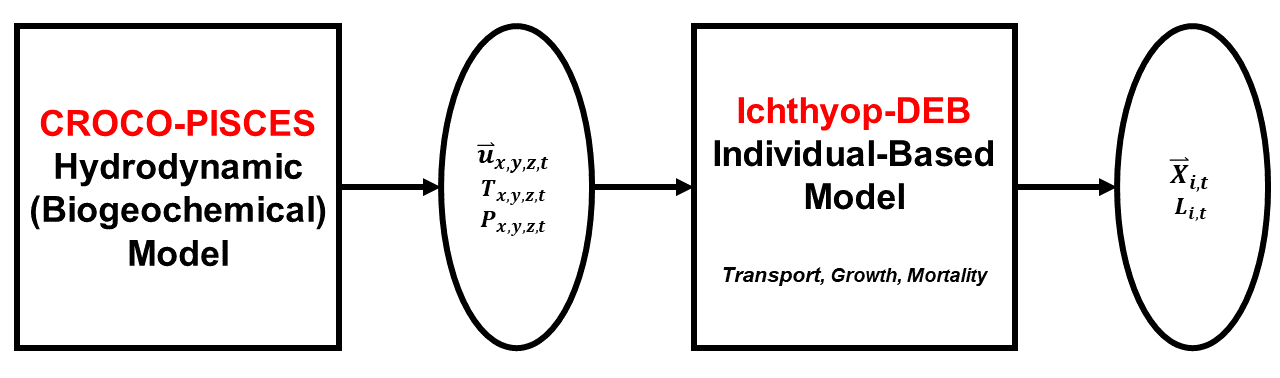
\includegraphics[width=1.0\textwidth]{figures/Chap3Ichthyop-DEB.png}
	\centering
	\caption{Representative flow diagram of the Ichthyop-DEB model and its hydrodynamic-biogeochemical forcing using CROCO-PISCES.}
	\label{Chap3Ichthyop-DEB}
\end{figure}

\subsection{Design concepts}

\begin{itemize}

\item Observation: A spatio-temporal recruitment index was computed for each simulation and compared with egg presence observational data. Three recruitment criterions were tested, either based on 30-day retention over the continental shelf (\gls{cri1}), retention until the larval length reach 2 $cm$ (\gls{cri2}) and mortality-weighted larval worth until the larval length reach 2 $cm$ (\gls{cri3}). Standard length of a larva used for criterion \gls{cri2} and \gls{cri3} relates to its structural volume as follows:\\

\begin{equation}
	L_{w} = \frac
				{V^{1/3}}
				{\delta_{M}}
	\label{L_W}
\end{equation}\\

where $L_{w}$ is the physical standard length ($cm$), $V$ is the structural volume ($cm^3$) 
and $\delta_{M}$ is a shape coefficient.\\

\end{itemize}

\subsection{Initialization}
In each simulation, individuals were released randomly along the coastal spawning area (Fig. \ref{Chap3SpawningZone}) each month at days 1, 10 and 20, during the three climatological years used. The coastal spawning area was defined as the volume of water between latitudes 2\textdegree $S$ and 20\textdegree $S$, depth range [0 - 45 $m$] and from the coast to isobath 2000 $m$.\\

The initial values of the bioenergetic variables for each individual were set as initial reserve $E0=1J$ and initial structure $V0=0.000001cm^3$. Formally, an egg is only composed of reserve but in practice a very small value for $V0$ value was needed in order to avoid division by zero in the mobilization equation. We checked that a value of $V0$ larger by one order of magnitude did not change the results.\\

\begin{figure}[ht]
	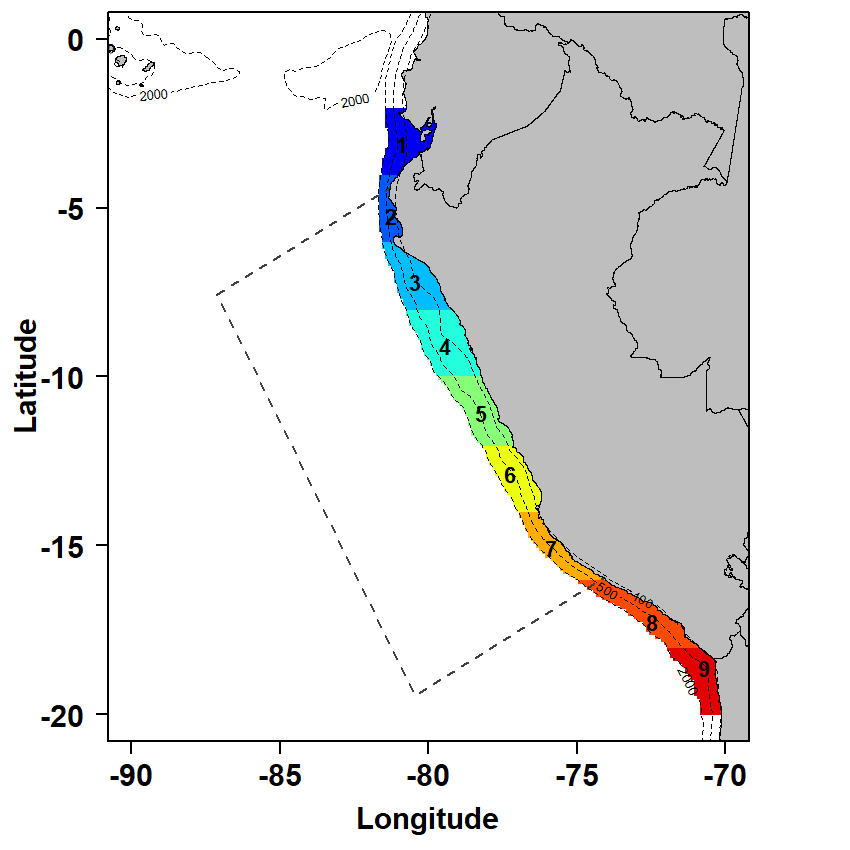
\includegraphics[width=1.0\textwidth]{figures/Chap3SpawningZone.png}
	\centering
	\caption{Model domain at 10 km of spatial resolution ($D01$). Spawning areas (1 - 9) are every 2\textdegree degrees of latitude between 2\textdegree $S$ and 20\textdegree $S$. Three isobaths (100 $m$, 500 $m$ and 2000 $m$) are shown.}
	\label{Chap3SpawningZone}
\end{figure}

\subsection{Sub-models}

\begin{itemize}

\item Growth: The \acrshort{deb} theory \citep{Kooi2009} was used to simulate the growth of larvae. It describes the acquisition and utilization of energy for metabolic processes during the complete life cycle of an organism depending on temperature ($T$) and food conditions ($f$). Here, this model was used to simulate larval growth through the description of energy reserve and body structure complexity evolution; maturation and reproduction processes were not considered. Energy assimilated from food in the environment is allocated partly to reserve for somatic maintenance ($E$), and the excess energy is used to increase the structure ($V$), i.e., physical length (see eqn. \ref{L_W}). The following system of ordinary differential equations describe the dynamics of $E$ (eqn. \ref{dEdt}) and $V$ (eqn. \ref{dVdt}).\\

Each parameter may be identified from specific observations for any species. In the absence of observations for the Peruvian anchovy (\textit{\gls{ringens}}), we used here parameters estimated for the European anchovy (\textit{\gls{encrasicolus}}, \cite{PethRoos2013}	, Table \ref{TabDEBparEncra}), a taxonomically close species that is also distributed in upwelling zones. $\left \{ \dot{p}_\mathrm{Am} \right \}$ is the surface-area-specific maximum assimilation rate, $\left [ \dot{p}_{M} \right ]$ is the specific volume-linked somatic maintenance rate, $\kappa$ is the fraction of mobilized reserve allocated to soma, ${\left [ E_{G} \right ]}$ is the volume-specific costs of structure and $\dot{p}_{C}$ (eqn. \ref{pC}) is a compound parameter corresponding to the mobilization of energy for maintenance,\\

\begin{equation}
	\dot{p}_{C} = \frac
					   {E\left ( \left [ E_{G} \right ] \frac{C_{T}\left \{ \dot{p}_\mathrm{Am} \right \}}{\left [ E_{m} \right ]} V^{-\frac{1}{3}}+\left [ \dot{p}_{M} \right ]\right )}
					   {\kappa\left ( \frac{E}{V} \right ) + \left [ E_{G} \right ]}
	\label{pC}
\end{equation}\\

where $\left[ E_{m} \right]$ is the maximum reserve density and $fC_{T}\left \{ \dot{p}_\mathrm{Am} \right \}V^{\frac{2}{3}}$ corresponds to the assimilation of energy which begins after birth, based on the following food concentration functional response (eqn. \ref{funct_response}),\\

\begin{equation}
	f = \frac{X}
			 {X+K}
    \label{funct_response}
\end{equation}\\

with $X$ the local food concentration (here meso-zooplankton fields coming from CROCO-PISCES), $K$ the half-saturation constant fixed with a value of 1.6 and $C_{T}$ a non-monotonic temperature correction factor. The parameter $C_{T}$ is defined as follows:\\

\begin{equation}
	C_{T} = exp\left ( \frac{T_{A}}{T_{1}} - \frac{T_{A}}{T} \right )
	\left ( \frac
				{1+exp\left ( \frac{T_{AL}}{T_{1}} - \frac{T_{AL}}{T_{L}} \right )
				  +exp\left ( \frac{T_{AH}}{T_{H}} - \frac{T_{AH}}{T_{1}} \right )}
				{1+exp\left ( \frac{T_{AL}}{T} - \frac{T_{AL}}{T_{L}} \right )
				  +exp\left ( \frac{T_{AH}}{T_{H}} - \frac{T_{AH}}{T} \right )}
	\right )
    \label{C_T}
\end{equation}\\

\begin{equation}
	\frac{dE}{dt} = f C_{T} \left \{ \dot{p}_\mathrm{Am} \right \} V^{\frac{2}{3}} - \dot{p}_{C}
	\label{dEdt}
\end{equation}\\

\begin{equation}
	\frac{dV}{dt} = \frac
						{\kappa \dot{p}_C - C_{T} \left [ \dot{p}_{M} \right ] V}
						{\left [ E_{G} \right ]}
	\label{dVdt}
\end{equation}\\

where $T$ is the water temperature surrounding an individual (coming from CROCO-PISCES), $T_{1}$ is the reference temperature (for which flux parameters were estimated), $T_{A}$ is the Arrhenius temperature \citep{Kooi2009} and $T_{AL}$, $T_{AH}$, $T_{L}$, $T_{H}$ are constants used to define a curved shape of the temperature correction according to temperature.\\

\item Recruitment: We considered two criteria for larval recruitment, hereafter referred to as the
age- and size-criterion, respectively. For the age-criterion (\gls{cri1}), an individual was considered
as recruited if it was within the coastal zone (offshore limit 2000 $m$ isobath) at age 30
$days$, like in the previous modelling study \citep{BrocLett2008}. For the size-criterion (\gls{cri2}), an individual was considered as recruited when it was within the coastal zone at a size larger
than 20 $mm$. The 20 $mm$ threshold was chosen because Peruvian anchovy larvae reached
an average size of 20 $mm$ at 30 $days$ \citep{CastHern2000, MoreClar2011, RiouOfel2021, OfelMoya2023}.\\

\item Mortality: We used the concept of super-individual \citep{ScheBave1995, ParrEvan2008} by assigning an initial worth of 1 to each individual, then applying a constant daily mortality rate until the age at recruitment, which we will call \gls{cri3}. The daily mortality rate was set to $0.1 d^{-1}$ as proposed for anchovies \citep{BailHoud1989, Houd2008}. The formula used to construct mortality is as follows: $(1-0.1)^{age}$, where $age$ is ``age at recruitment'', thus, individuals who recruit earlier will have a higher value than those who take longer, as shown in Fig. \ref{Chap3MortalityCurve}.

\end{itemize}

\begin{figure}[ht]
	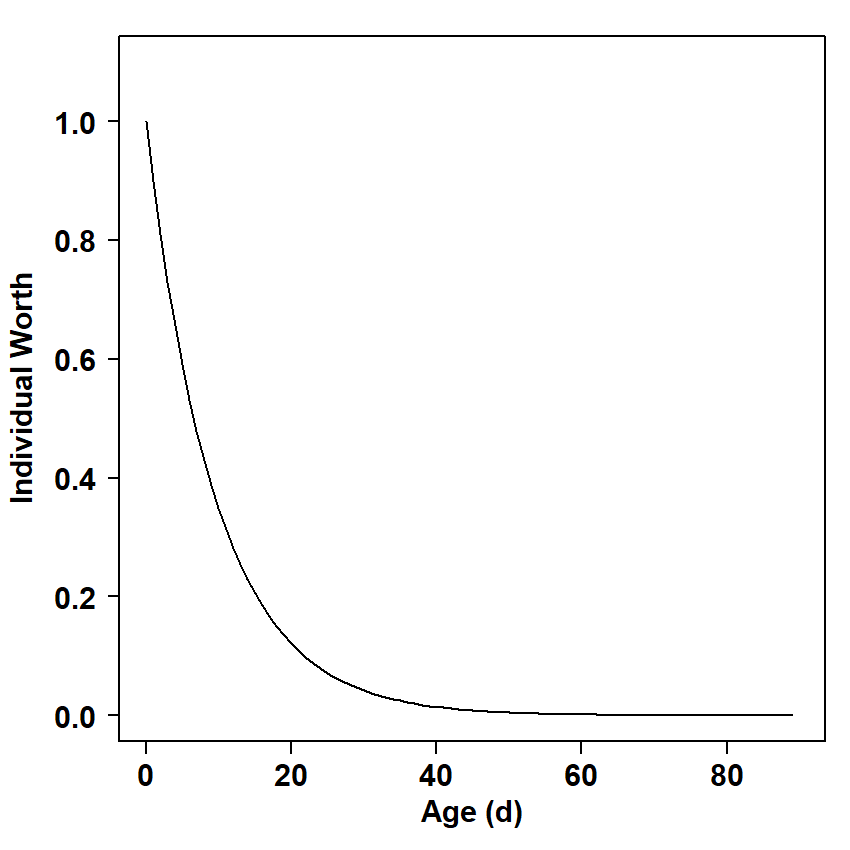
\includegraphics[width=1.0\textwidth]{figures/Chap3MortalityCurve.png}
	\centering
	\caption{The worth of an individual is a function of age, with a constant mortality rate of $0.1 d^{-1}$.}
	\label{Chap3MortalityCurve}
\end{figure}

\begin{landscape}
\begin{table}[H]
\centering
\begin{adjustbox}{width=1.0\textwidth}
\small
\begin{NiceTabular}{c|c|c|c|c|c|c|c}
\hline
                     &
    \textbf{$Sim 4$} &
    \textbf{$Sim 5$} &
    \textbf{$Sim 6$} &
    \textbf{$Sim 7$} &
    \textbf{$Sim 8$} &
    \textbf{$Sim 9$} &
    \textbf{$Sim 10$} \\
\hline
\makecell{Configuration \\ domain} &
	$D01$  		     &
	$D01$ 		     &
	$D01$ 			 &
	$D01$			 &
	$D01$			 &
	$D01$			 &
	$D01$			 \\
\makecell{CROCO \\ configuration}   		   &
	$22$\textdegree $S$ to $5$\textdegree $N$ &
	$22$\textdegree $S$ to $5$\textdegree $N$ &
	$22$\textdegree $S$ to $5$\textdegree $N$ &
	$22$\textdegree $S$ to $5$\textdegree $N$ &
	$22$\textdegree $S$ to $5$\textdegree $N$ &
	$22$\textdegree $S$ to $5$\textdegree $N$ &
	$22$\textdegree $S$ to $5$\textdegree $N$ \\
Forcing type &
	\makecell{Physical \& \\biogeochemical} &
	\makecell{Physical \& \\biogeochemical} &
	\makecell{Physical \& \\biogeochemical} &
	\makecell{Physical \& \\biogeochemical} &
	\makecell{Physical \& \\biogeochemical} &
	\makecell{Physical \& \\biogeochemical} &
	\makecell{Physical \& \\biogeochemical} \\
Bathymetry source &
	STRM30 &
	STRM30 &
	STRM30 &
	STRM30 &
	STRM30 &
	STRM30 &
	STRM30 \\
\makecell{Horizontal \\ grid resolution} &
	$10 km$                  &
	$10 km$                  &
	$10 km$                  &
	$10 km$                  &
	$10 km$                  &
	$10 km$                  &
	$10 km$                  \\
\makecell{Latitudinal \\ spawning range}     &
	$2$\textdegree $S$ - $20$\textdegree $S$ &
	$2$\textdegree $S$ - $20$\textdegree $S$ &
	$2$\textdegree $S$ - $20$\textdegree $S$ &
	$2$\textdegree $S$ - $20$\textdegree $S$ &
	$2$\textdegree $S$ - $20$\textdegree $S$ &
	$2$\textdegree $S$ - $20$\textdegree $S$ &
	$2$\textdegree $S$ - $20$\textdegree $S$ \\					
\makecell{Growth \\ sub-model} &
	No  &
	Yes &
	Yes &
	Yes &
	Yes &
	Yes &
	Yes \\
\makecell{Recruitment \\ criterion evaluated \tabularnote{Recruitment criterion 1: retention at 30 days; 2: retention at 20 mm; 3: retention at 20 mm with constant mortality.}}  &
	1       &
	2 and 3 &
	2 and 3 &
	2 and 3 &
	2 and 3 &
	2 and 3 &
	2 and 3 \\
Correction temperature \tabularnote{Temperature correction factor Case 1: $T_{H} = 294 K$($=21$\textdegree $C$) and $T_{AH} = 95000 K$; Case 2: $T_{H} = 297 K$($=24$\textdegree $C$) and $T_{AH} = 570000 K$} &
	-      &
	Case 1 &
	Case 2 &
	Case 1 &
	Case 2 &
	Case 1 &
	Case 2 \\
\makecell{Food half \\ saturation constant \\ ($K$)}  &
	- 	&
	1.6 &
	1.6 &
	0   &
	0   &
	1.6 &
	1.6 \\
Mortality &
	-   &
	Yes &
	Yes &
	Yes &
	Yes &
	Yes &
	Yes \\
Temporal scale  &
	Climatology &
	Climatology &
	Climatology &
	Climatology &
	Climatology &
	Interannual &
	Interannual \\
\hline
\end{NiceTabular}
\end{adjustbox}
\caption{Summary of simulations performed to study recruitment predictions sensitivity. This table list all parameters that differ between simulations.}
\label{TabSimusChap3}
\end{table}
\end{landscape}

%\begin{landscape}
\begin{table}[H]
\centering
\begin{adjustbox}{width=1.0\textwidth}
\begin{tabular}{l|l|l|l}
\hline
\multicolumn{4}{l}{Primary parameters (rates are at reference temperature $T_{1} = 293 K$  ($=20$\textdegree $C$)} \\
\hline
Symbol   & Value        & Unit & Definition                                \\
\hline
$L_{h}$  & 0.28         & $cm$ & Hatch length                              \\
$L_{b}$  & 0.35         & $cm$ & Yolk-sac to feeding larva threshold       \\
$T_{A}$  & 9800         & $K$  & Arrhenius temperature                     \\
$T_{L}$  & 279/279      & $K$  & Lower temperature boundary                \\
$T_{H}$  & 294/297      & $K$  & Upper temperature boundary                \\
$T_{AL}$ & 20000/20000  & $K$  & Arrhenius temperature for lower boundary  \\
$T_{AH}$ & 95000/570000 & $K$  & Arrhenius temperature for upper boundary   \\
$K$      & 1.6          & $\mu mol CL^{-1}$ & Half-saturation constant       \\
$\kappa_{\mathrm{x}}$   & 0.71 & - & Fraction of food energy fixed in reserve \\
$\left\{\dot{p}_\mathrm{Xm} \right\}$
	& 516
	& $J.cm^{-2}.d^{-1}$
	& Maximum surface-specific ingestion rate         \\
$\left[E_{m} \right]$
	& 2700 
	& $J.cm^{-3}$
	& Maximum reserve density                         \\
$\left[E_{G} \right]$
	& 4000
	& $J.cm^{-3}$
	& Volume-specific costs of structure              \\
$\left[\dot{p}_{M} \right]$
	& 76.22 
	& $J.cm^{-3}.d^{-1}$
	& Volume-specific somatic maintenance rate\\
$\kappa$
	& 0.7
	& - 
	& \makecell[l]{Fraction of mobilized reserve allocated to \\ growth and somatic maintenance} \\
\hline
\multicolumn{4}{l}{Auxiliary and Compounds parameters}   \\
\hline
Symbol & Value & Unit & Definition                   \\
$\delta_{M}$
	& 0.152
	& -
	& Shape coefficient                               \\
$\left \{ \dot{p}_\mathrm{Am} \right \}$
	& $\kappa_{\mathrm{x}} $ $\left \{ \dot{p}_\mathrm{Xm} \right \}=366$
	& $J.cm^{-2}.d^{-1}$
	& Maximum surface-area-specific assimilation rate\\
\hline
\end{tabular}
\end{adjustbox}
\caption{Parameters used for the bioenergetic model describing larval growth. These values were estimated by \cite{PethRoos2013} for \textit{\gls{encrasicolus}}, except half saturation constant ($K$), estimated for the current configuration and fixed at 1.6 $\mu mol CL^{-1}$. Comparison with data showed that these parameters allowed to reproduce \textit{\gls{ringens}} larval growth. The values of $T_{L}$, $T_{H}$, $T_{AL}$, $T_{AH}$ are detailed for Case 1 and Case 2 respectively (see Table \ref{TabSimusChap3}). Although these parameters were originally calibrated with a reference temperature of 16\textdegree $C$, in order to standardize the comparison with other species, we expressed them at 20\textdegree $C$.}
\label{TabDEBparEncra}
\end{table}
%\end{landscape}

\subsection{Simulations and sensitivity analysis}

Table \ref{TabSimusChap3} shows seven simulations named from $Sim4$ to $Sim10$ performed in order
to explore the model sensitivity to different environmental forcing fields and larval growth
parameters using the $D01$ grid and the larval size threshold (20 $mm$) as a criterion for
recruitment (size-criterion). The \acrshort{deb} parameters values are given in Table \ref{TabDEBparEncra}, corresponding to \textit{\gls{encrasicolus}} \citep{PethRoos2013} but fitting \textit{\gls{ringens}} larval growth well. In order to disentangle the effects of food and temperature on growth, and ultimately on recruitment, simulations were repeated using a half saturation parameter either null, i.e., $f = 1$ (no food limitation) or calculated such that $f = 0.5$ for the average meso-zooplankton concentration over the continental shelf off Peru with a half saturation constant of $K = 1.6$. To contrast the effect of temperature on growth, we used two different shapes for the curve of the energy fluxes temperature correction ($C_{T}$; Fig. \ref{Chap3CT_curves}). In both cases, $C_{T}$ dropped to very low values for temperature higher than $25$\textdegree $C$ but in the first case the maximum value of $C_{T}$ was at $19$\textdegree $C$ and then it dropped slowly (hereafter referred to as ``Case 1'') whereas in the second case the maximum was at 23 \textdegree C and then it dropped quickly (hereafter referred to as ``Case 2''). These temperature thresholds were chosen to fit \textit{\gls{ringens}} distribution in Peru \citep{CastPena2022}. Two additional simulations were conducted under the same configuration as cases 1 and 2, with an interannual forcing. The objective was to explore recruitment on a different time scale than the climatological one. All simulations lasted 90 days, a value found from preliminary simulations as long enough for the slowest growing individuals to reach the recruitment size. Larval retention at 30 days (age criterion, $Sim 4$) was also compared with the size-criterion in all four simulations ($Sim 5$, $Sim 6$, $Sim 7$ and $Sim 8$). In order to quantify the variation of results between simulations with ($Sim 5$, $Sim 6$) and without ($Sim 7$, $Sim 8$) food limitation, we calculated the percentage of variation, e.g. ($\frac{Sim 7-Sim 5}{Sim 5*100}$)

\begin{figure}[ht]
	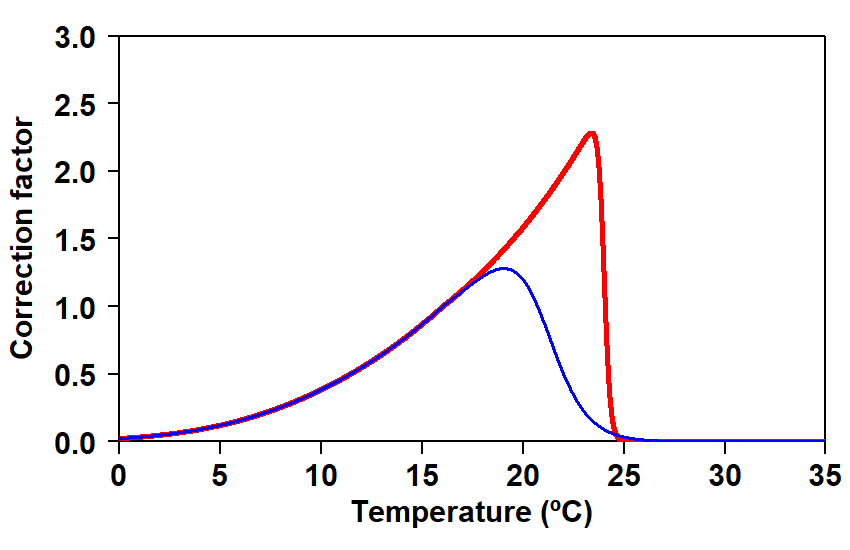
\includegraphics[width=1.0\textwidth]{figures/Chap3CT_curves.png}
	\centering
	\caption{Temperature correction curves for the metabolic flux in the dynamic energy budget model (eqn. \ref{C_T}); blue and red curve correspond respectively to Case 1 and Case 2 in Table 1.}
	\label{Chap3CT_curves}
\end{figure}

\subsection{Ichthyop-DEB model coupling implementation}\label{Chap3Ich-DEBstd}

Jorge Flores-Valiente et al.\\

The following description is a simplification of the \gls{encrasicolus} \acrshort{deb} model developed by \cite{PethRoos2013} as we only focus on the embryo and larva stages. We implemented these equations in the Lagrangian tool routines of \gls{ich} \citep{LettVerl2008} to develop \gls{ich-deb}.\\

\begin{figure}[ht]
	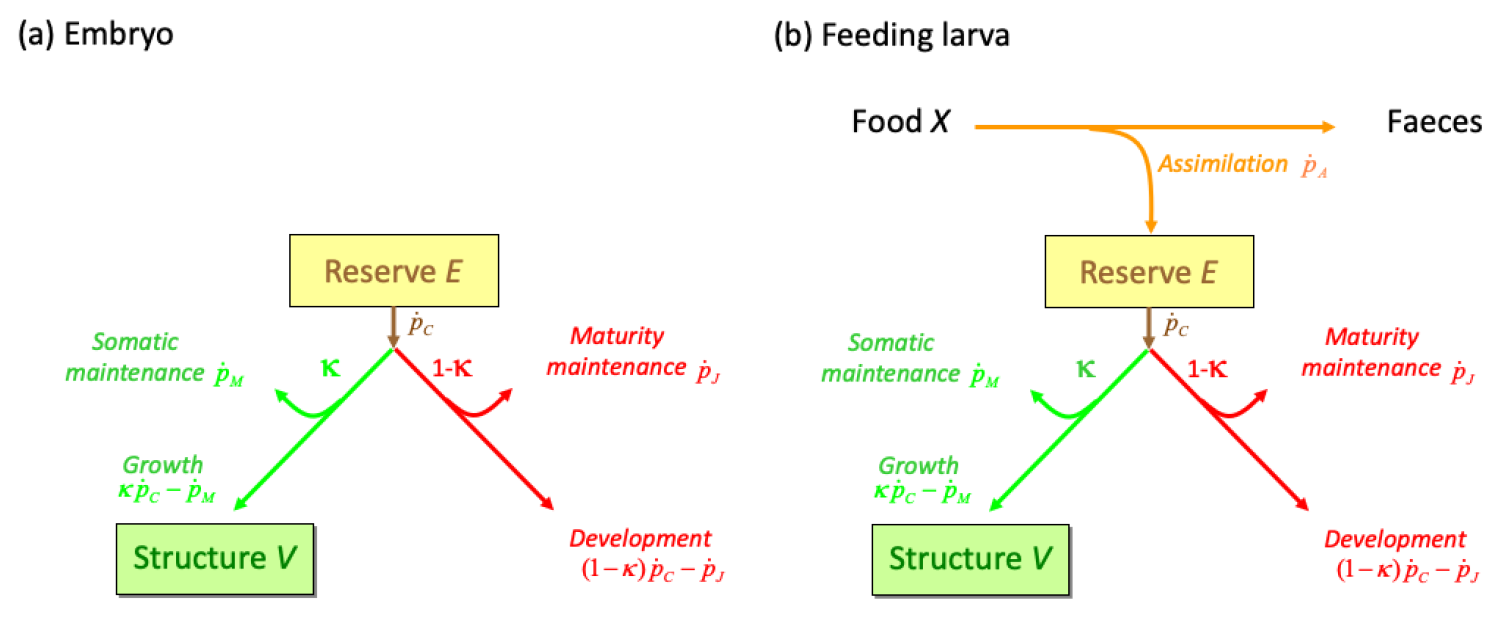
\includegraphics[width=1.0\textwidth]{figures/Chap3DEBflux.png}
	\centering
	\caption{Schemes of the energy fluxes of a \acrlong{deb} model (a) for the embryo stage (non-feeding stage) and (b) the feeding larval stage.}
	\label{Chap3DEBflux}
\end{figure}

\subsubsection{Forcing variables}\label{Chap3ForVar}
\hfill \\

$T$ Temperature ($K$) is the water temperature surrounding an individual (modeled by CROCO-PISCES)\\

$X$ Food density averaged Mesozooplankton field ($\left[ \mu mol CL^{-1} \right]$) over the water column (modeled by CROCO-PISCES)\\

\subsubsection{Initial conditions of state variables (egg stage)}\label{Chap3InitCond}

The age of the individual is set at zero on the day of spawning.\\

\begin{tabular}{|c|c|c|c|}
\hline 
Symbol  & Value      & Units  & Definition      \\ 
\hline 
$E$     & $0.99$     & $J$    & Initial Reserve \\ 
$V$     & $0.000001$ & $mm^3$ & Initial Structure\\
\hline 
\end{tabular} 

\subsubsection{Primary parameters}\label{Chap3PriPar}

\begin{table}[H]
\centering
\begin{adjustbox}{width=1.2\textwidth}
\begin{tabular}{l|l|l|l}
\hline
\multicolumn{4}{l}{Primary parameters (rates are at reference temperature $T_{1} = 293 K$  ($=20$\textdegree $C$)} \\
\hline
Symbol   & Value        & Unit & Definition                                \\
\hline
$L_{h}$  & 0.28         & $cm$ & Hatch length                              \\
$L_{b}$  & 0.35         & $cm$ & Yolk-sac to feeding larva threshold       \\
$T_{A}$  & 9800         & $K$  & Arrhenius temperature                     \\
$T_{L}$  & 279/279      & $K$  & Lower temperature boundary                \\
$T_{H}$  & 294/297      & $K$  & Upper temperature boundary                \\
$T_{AL}$ & 20000/20000  & $K$  & Arrhenius temperature for lower boundary  \\
$T_{AH}$ & 95000/570000 & $K$  & Arrhenius temperature for upper boundary   \\
$K$      & 1.6          & $\mu mol CL^{-1}$ & Half-saturation constant       \\
$\kappa_{\mathrm{x}}$   & 0.71 & - & Fraction of food energy fixed in reserve \\
$\left\{\dot{p}_\mathrm{Xm} \right\}$
	& 516
	& $J.cm^{-2}.d^{-1}$
	& Maximum surface-specific ingestion rate         \\
$\left[E_{m} \right]$
	& 2700 
	& $J.cm^{-3}$
	& Maximum reserve density                         \\
$\left[E_{G} \right]$
	& 4000
	& $J.cm^{-3}$
	& Volume-specific costs of structure              \\
$\left[\dot{p}_{M} \right]$
	& 76.22 
	& $J.cm^{-3}.d^{-1}$
	& Volume-specific somatic maintenance rate\\
$\kappa$
	& 0.7
	& - 
	& Fraction of mobilized reserve allocated to growth and somatic maintenance    \\
\hline
\end{tabular}
\end{adjustbox}
\end{table}

\subsubsection{Auxiliary and compounds parameters}

\begin{table}[H]
\centering
\begin{adjustbox}{width=1.2\textwidth}
\begin{tabular}{l|l|l|l}
\hline
\multicolumn{4}{l}{Auxiliary and Compounds parameters}   \\
\hline
Symbol & Value & Unit & Definition                   \\
$\delta_{M}$
	& 0.152
	& -
	& Shape coefficient                               \\
$\left \{ \dot{p}_\mathrm{Am} \right \}$
	& $\kappa_{\mathrm{x}} $ $\left \{ \dot{p}_\mathrm{Xm} \right \}=366$
	& $J.cm^{-2}.d^{-1}$
	& Maximum surface-area-specific assimilation rate\\
\hline
\end{tabular}
\end{adjustbox}
\end{table}

\subsubsection{Scaled functional response}\label{Chap3resp_f}
\hfill \\

$V_{b} = (\delta_{M}L_{b})^3$ \hfill Structural volume at first-feeding in $cm^3$.\\

\textbf{if} $(V < V_{b})$ \\

$f = 0$ \hfill No feeding.\\

\textbf{else}\\

$f= \frac{X}{X+K}$	    \hfill Feeding.\\

\subsubsection{Temperature correction}\label{Chap3cT_corr}
\hfill \\

Each rate parameter is corrected for temperature according to the following equation \citep{Kooi2009}.\\

$
	C_{T} = exp\left ( \frac{T_{A}}{T_{1}} - \frac{T_{A}}{T} \right )
	\left ( \frac
				{1+exp\left ( \frac{T_{AL}}{T_{1}} - \frac{T_{AL}}{T_{L}} \right )
				  +exp\left ( \frac{T_{AH}}{T_{H}} - \frac{T_{AH}}{T_{1}} \right )}
				{1+exp\left ( \frac{T_{AL}}{T} - \frac{T_{AL}}{T_{L}} \right )
				  +exp\left ( \frac{T_{AH}}{T_{H}} - \frac{T_{AH}}{T} \right )}
	\right )
$\\

With $T_{1}$ the reference temperature (at which flux parameters were estimated), $T_{A}$ is the Arrhenius temperature and $T_{AH}$, $T_{AH}$, $T_{L}$, $T_{H}$ are constants used to define a curved shape of the temperature correction according to temperature.\\

$\left \{ \dot{p}_\mathrm{Am} \right \}_{T} = C_{T} \left \{ \dot{p}_\mathrm{Am} \right \}_{T_{1}}$\\

$\left [ \dot{p}_{M} \right ]_{T} = C_{T} \left [ \dot{p}_{M} \right ]_{T_{1}}$\\

\subsubsection{Fluxes ($Jd^{-1}$)}\label{Chap3Fluxex}
\hfill \\

$\dot{p}_\mathrm{A} = f \left \{ \dot{p}_\mathrm{Am} \right \}_{T} V^{2/3}$ \hfill Assimilation.\\

$\dot{p}_\mathrm{M} = \left [ \dot{p}_{M} \right ]_{T} V$ \hfill Volume-related somatic maintenance.\\


	$\dot{p}_{C} = \frac
					   {E\left ( \left [ E_{G} \right ] \frac{C_{T}\left \{ \dot{p}_\mathrm{Am} \right \}_{T}}{\left [ E_{m} \right ]} V^{-\frac{1}{3}}+\left [ \dot{p}_{M} \right ]_{T}\right )}
					   {\kappa\left ( \frac{E}{V} \right ) + \left [ E_{G} \right ]}$ \hfill Mobilization of energy.\\

$\dot{p}_{G} = \kappa \dot{p}_{C} - \dot{p}_\mathrm{M}$ \hfill Energy directed to structural growth.\\

$\dot{p}_{J} = V \frac{\left ( 1 - \kappa \right )}{\kappa}\left [ \dot{p}_{M} \right ]_{T}$ \hfill Maturity maintenance (for $V < V_{p}$ (Structural volume at puberty), the condition is always TRUE because in \gls{ich-deb} the complexity level of the organism at puberty is never exceeded, as we only consider embryos and larvae).\\

Starvation test\\

\textbf{if} $\kappa \dot{p}_{C} < \dot{p}_\mathrm{M}$ or $\left ( 1- \kappa \right ) \dot{p}_{C} < \dot{p}_{J}$\\

$starvation = 1$ \hfill Individual (or super-individual) removed from population.\\

\textbf{else}\\

$starvation = 0$ \hfill Individual continues in the simulation.\\

\subsubsection{Differential equations}\label{Chap3DiffEq}
\hfill \\

$\frac{dE}{dt} = \dot{p}_\mathrm{A} - \dot{p}_{C}$ \hfill Reserve dynamics.\\

$\frac{dV}{dt} = \frac{\dot{p}_{G}}{\left[ E_{G} \right]}$ \hfill Structure dynamics.\\

\subsubsection{Integration}\label{Chap3Integ}
\hfill \\

$E\left ( t + \Delta t \right ) = E\left ( t \right ) + \frac{dE}{dt}\Delta t$ \\

$V\left ( t + \Delta t \right ) = V\left ( t \right ) + \frac{dV}{dt}\Delta t$ \\

With $\Delta t = 0.083 d \left (=2hours\right )$

\subsubsection{Observable variables}\label{Chap3ObsVar}
\hfill \\

$L_{w} = \frac{V^{1/3}}{\delta_{M}}$ \hfill Physical length ($cm$).\\

where $L_{w}$ is the standard length $SL$ ($cm$), $V$ the structural volume ($cm^3$) and $\delta_{M}$ a shape coefficient.\\

We assume that the larva does not change in shape till it reaches our length criteria of $2cm$ (SL) and that there is a constant proportionality ($\delta_{M}$) between structural volume and length.\\


\clearpage
\section{Results of climatological simulations}\label{Chap3Resu1}

In general, the bioenergetic model of European anchovy (\textit{\gls{encrasicolus}}), developed by \cite{PethRoos2013}, simulated well the larval growth patterns of \textit{\gls{ringens}} for different temperatures and compared with individuals reared in the laboratory (15, 18, 19 \textdegree C, \cite{RiouOfel2021}) and individuals sampled from the natural environment (16ºC, \cite{MoreClar2011}). The average simulated growth (colored solid lines) demonstrates an acceptable fit to laboratory and literature data, as shown in Fig. \ref{Chap3DEBvsData}.

\begin{figure}[H]
	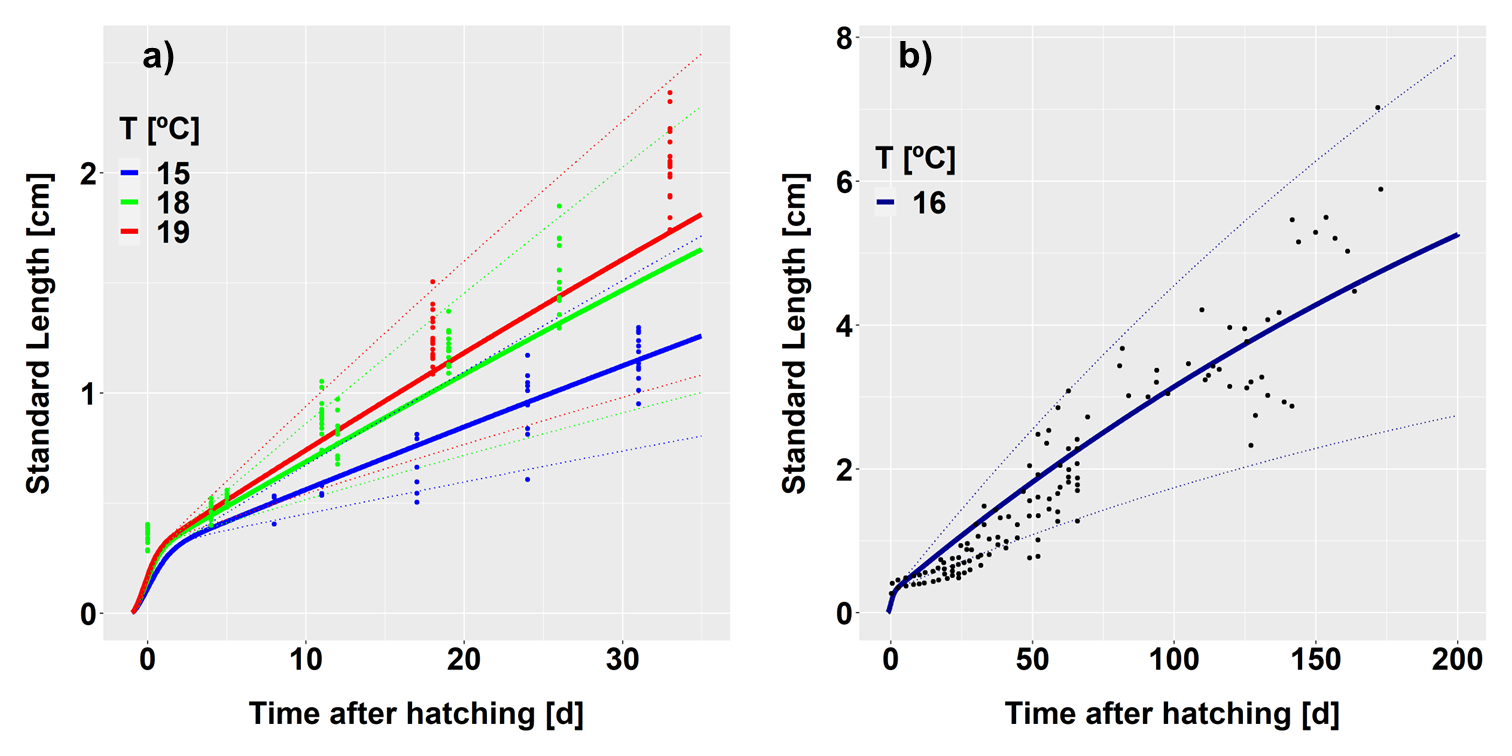
\includegraphics[width=1.0\textwidth]{figures/Chap3DEBvsData.png}
	\centering
	\caption{Comparison of Peruvian anchovy simulated larval growth and laboratory
observations from \cite{RiouOfel2021} (a) and in situ observations from \cite{MoreClar2011}
(b). Thick lines correspond to average size predictions considering ten $f$ values from 0.1 to 1
with 0.1 steps (food limitation factor, see section \ref{Chap3Ich-DEBstd}) at 19°C (red), 18°C (green) and 15°C (blue) in (a) and at 16°C in (b). Dotted lines correspond to standard deviation of the simulated larval growth. Colored dots show the corresponding observations. The bioenergetic model
parameters were taken from \cite{PethRoos2013}. Note that the scales are different in the
two panels.}
	\label{Chap3DEBvsData}
\end{figure}

Globally, in $Sim 4$ we obtained similar retention patterns as \cite{BrocLett2008}, who used different physical forcing fields. The interaction of spawning depth and month displayed the same characteristic pattern, with highest retention in austral winter for the superficial spawning depth level (0 - 15 $m$) and in summer for the deepest spawning levels (30 - 45 $m$; bars in Fig. \ref{Chap3BrocVSFloreBarplots}). We also found the same seasonal trends when the spawning area was split into inner shelf (0 - 100 $m$ isobaths) and offshore shelf (100 - 500 $m$ and 500 - 2000 $m$ isobaths; lines in Fig. \ref{Chap3BrocVSFloreBarplots}). The results differed most in the zone between 14\textdegree S to 16\textdegree S with highest values obtained from July to October in \cite{BrocLett2008}, as opposed to a maximum in January-February obtained here (Fig. \ref{Chap3BrocVSFloreHovmuller}).\\

\begin{figure}[H]
	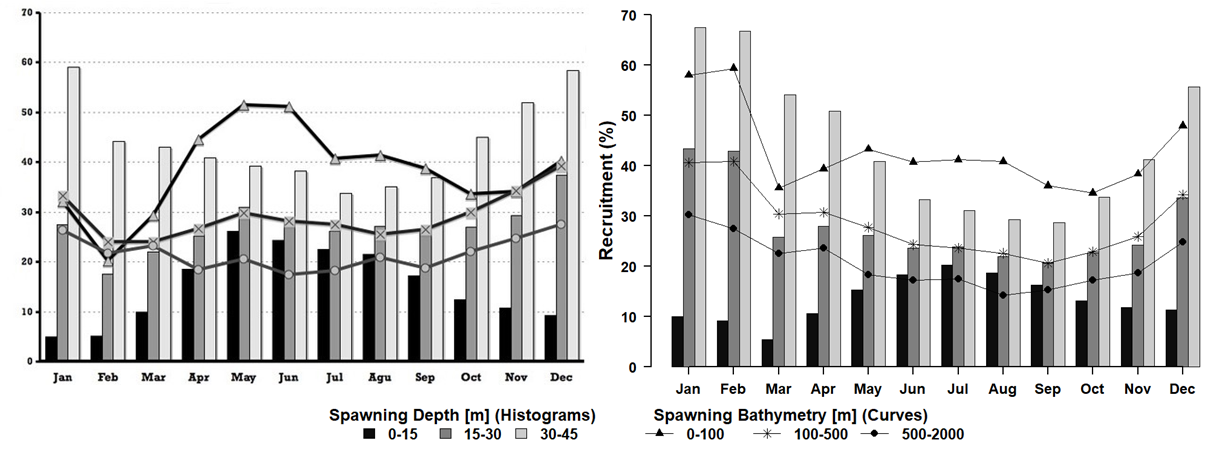
\includegraphics[width=1.0\textwidth]{figures/Chap3BrocVSFloreBarplots.png}
	\centering
	\caption{Percentage of recruited larvae of Peruvian anchovy obtained for different spawning months, spawning depths, and isobaths delimiting spawning areas horizontally from \cite{BrocLett2008} (left) and from $Sim 4$ (right).}
	\label{Chap3BrocVSFloreBarplots}
\end{figure}

\begin{figure}[H]
	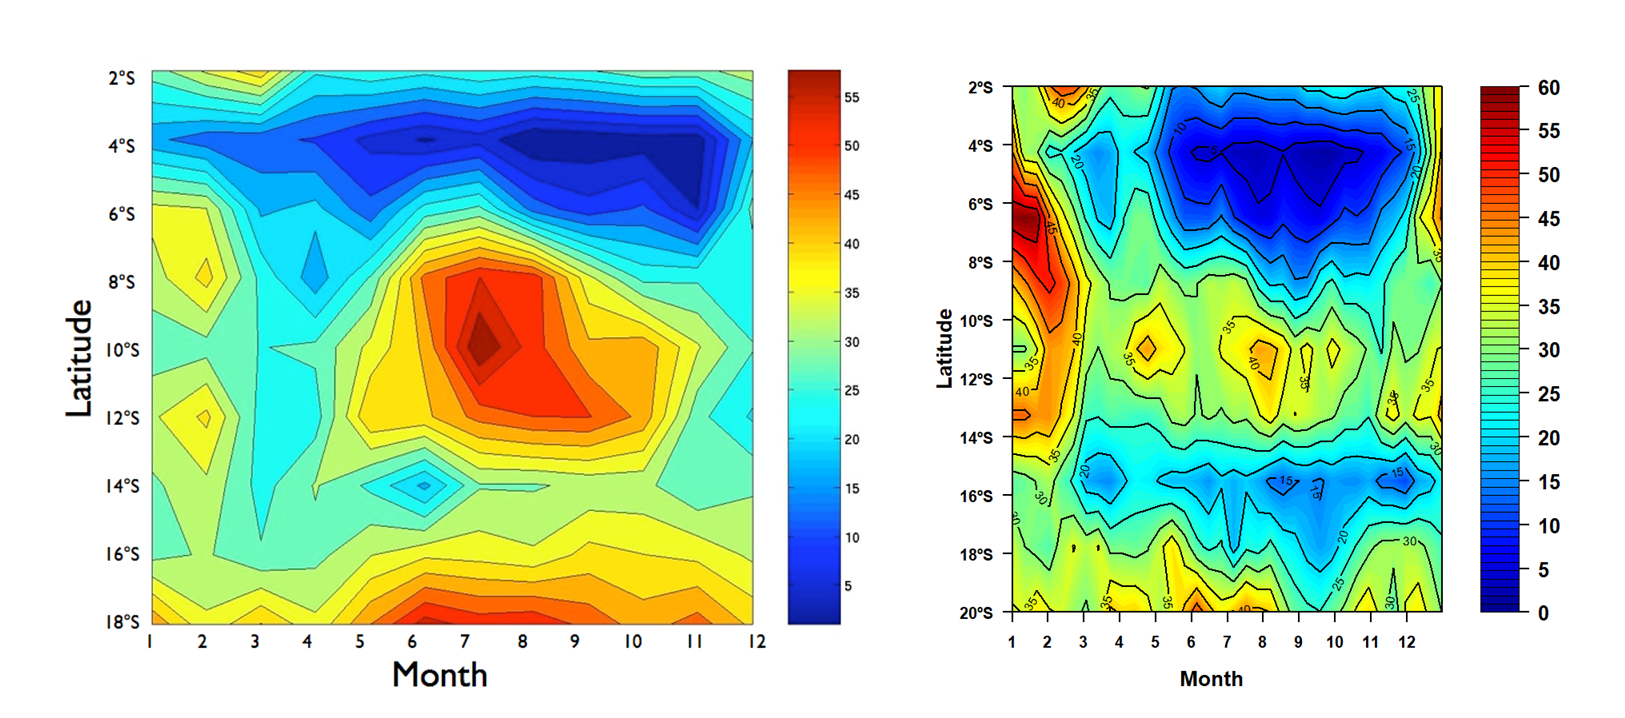
\includegraphics[width=1.0\textwidth]{figures/Chap3BrocVSFloreHovmuller.png}
	\centering
	\caption{Percentage of recruited larvae of Peruvian anchovy obtained for different months and latitudes from (left) \cite{BrocLett2008} and (right) $Sim 4$.}
	\label{Chap3BrocVSFloreHovmuller}
\end{figure}

The analysis of variance (ANOVA, Table \ref{ANOVAsim5}) applied to recruitment rates for Case 1 ($Sim 5$) indicates that spawning depth had the greatest effect on recruitment rates (28.35 \%), followed by latitude (14.26 \%). The other factors (spawning bathymetry, spawning month, and spawning year) showed less than 3 \% of the variance in recruitment rates. However, the combined effect of spawning month and spawning latitude explained 11.26 \% of the variance, followed by spawning month combined with spawning depth (9.20 \%). The remaining combinations did not exceed 4 \% percent explanation.\\

%\begin{landscape}
\begin{table}[H]
\centering
\begin{adjustbox}{width=0.9\textwidth}
\small
\begin{tabular}{c|r|r|r|r|r|r}
\hline
                                  &
	\textbf{Df}                   &
	\textbf{Sum Sq}               &
	\textbf{Mean Sq}              &
	\textbf{F-value}    		   &
	\textbf{Pr (\textgreater{F})} &
	$\mathbf{\% Exp}$      \\
\hline
Year                  & 2    & 594.61    & 297.31    & 3.71    & 0.02                & 0.02  \\
Month                 & 11   & 46972.03  & 4270.18   & 53.28   & 0.00                & 1.82  \\
Depth                 & 2    & 729892.48 & 364946.24 & 4553.68 & 0.00                & 28.35 \\
Bathymetry            & 2    & 77575.46  & 38787.73  & 483.98  & 0.00                & 3.01  \\
Latitude              & 8    & 367107.93 & 45888.49  & 572.58  & 0.00                & 14.26 \\
Year x Month          & 22   & 13008.37  & 591.29    & 7.38    & 0.00                & 0.51  \\
Year x Depth          & 4    & 355.96    & 88.99     & 1.11    & 0.35                & 0.01  \\
Year x Bathymetry     & 4    & 607.77    & 151.94    & 1.90    & 0.11                & 0.02  \\
Year x Latitude       & 16   & 9125.50   & 570.34    & 7.12    & 0.00                & 0.35  \\
Month x Depth         & 22   & 236883.93 & 10767.45  & 134.35  & 0.00                & 9.20  \\
Month x Bathymetry    & 22   & 32948.88  & 1497.68   & 18.69   & 0.00                & 1.28  \\
Month x Latitude      & 88   & 290053.41 & 3296.06   & 41.13   & 0.00                & 11.26 \\
Depth x Bathymetry    & 4    & 3913.28   & 978.32    & 12.21   & 0.00                & 0.15  \\
Depth x Latitude      & 16   & 78663.56  & 4916.47   & 61.35   & 0.00                & 3.06  \\
Bathymetry x Latitude & 12   & 108870.81 & 9072.57   & 113.20  & 0.00                & 4.23  \\
Residuals             & 7216 & 578313.56 & 80.14     &         &                     & 22.46 \\
\hline
\end{tabular}
\end{adjustbox}
\caption{ANOVA of recruitment rates for $Sim 5$ (Case 1).}
\label{ANOVAsim5}
\end{table}
%\end{landscape}

In Case 2 ($Sim 6$), the results of the ANOVA (Table \ref{ANOVAsim6}) indicated that spawning depth had the greatest effect on recruitment rates (20.71 \%), followed by latitude (13.19 \%) and month of spawning (9.48 \%). The remaining factors (spawning bathymetry and spawning year) collectively accounted for less than 5 \% of the variance. The combined effect of spawning month and latitude explained 8.77 \% of the variance, while the combined effect of spawning month and depth explained a value similar to the previous one (8.04 \%). Another noteworthy combination was that of bathymetry and spawning latitude (6.58 \%). The remaining combinations did not demonstrate particularly noteworthy values.\\

When we included larval growth ($Sim 5$ and $Sim 6$) and changed the criterion used for retention from age ($Sim 4$, 30 days, grey bars) to size ($Sim 5$ and $Sim 6$; $>$ 2 $cm$, black line) we obtained nearly identical results, except when mortality ($Sim 5$ and $Sim 6$; red line) was further included then small differences occurred in simulated recruitment patterns (Fig. \ref{Chap3Case1CriterionCompar} and Fig. \ref{Chap3Case2CriterionCompar}, respectively). In Case 1 ($Sim 5$), when the bio-energetic fluxes decayed smoothly at high temperature, the seasonal pattern remained similar using recruitment criteria 1,2 and 3 favoring summer months (Fig. \ref{Chap3Case1CriterionCompar}a). Latitudinal range between 6\textdegree - 14\textdegree S showed the highest recruitment value using recruitment criteria 1,2 but using criterion 3 only the zone between 6\textdegree - 8\textdegree $S$ was the most important (Fig. \ref{Chap3Case1CriterionCompar}b).\\

%\begin{landscape}
\begin{table}[H]
\centering
\begin{adjustbox}{width=0.9\textwidth}
\small
\begin{tabular}{c|r|r|r|r|r|r}
\hline
                                  &
	\textbf{Df}                   &
	\textbf{Sum Sq}               &
	\textbf{Mean Sq}              &
	\textbf{F-value}    		   &
	\textbf{Pr (\textgreater{F})} &
	$\mathbf{\% Exp}$      \\
\hline
Year                  & 2    & 645.96    & 322.98    & 3.09    & 0.05                & 0.02  \\
Month                 & 11   & 322491.73 & 29317.43  & 280.91  & 0.00                & 9.48  \\
Depth                 & 2    & 704668.20 & 352334.10 & 3375.96 & 0.00                & 20.71 \\
Bathymetry            & 2    & 163298.92 & 81649.46  & 782.34  & 0.00                & 4.80  \\
Latitude              & 8    & 448898.07 & 56112.26  & 537.65  & 0.00                & 13.19 \\
Year x Month          & 22   & 12459.78  & 566.35    & 5.43    & 0.00                & 0.37  \\
Year x Depth          & 4    & 744.83    & 186.21    & 1.78    & 0.13                & 0.02  \\
Year x Bathymetry     & 4    & 578.29    & 144.57    & 1.39    & 0.24                & 0.02  \\
Year x Latitude       & 16   & 10171.15  & 635.70    & 6.09    & 0.00                & 0.30  \\
Month x Depth         & 22   & 273637.25 & 12438.06  & 119.18  & 0.00                & 8.04  \\
Month x Bathymetry    & 22   & 31626.91  & 1437.59   & 13.77   & 0.00                & 0.93  \\
Month x Latitude      & 88   & 298338.78 & 3390.21   & 32.48   & 0.00                & 8.77  \\
Depth x Bathymetry    & 4    & 4990.27   & 1247.57   & 11.95   & 0.00                & 0.15  \\
Depth x Latitude      & 16   & 153670.06 & 9604.38   & 92.03   & 0.00                & 4.52  \\
Bathymetry x Latitude & 12   & 223998.82 & 18666.57  & 178.86  & 0.00                & 6.58  \\
Residuals             & 7216 & 753101.16 & 104.37    &         &                     & 22.13 \\
\hline
\end{tabular}
\end{adjustbox}
\caption{ANOVA of recruitment rates for $Sim 6$ (Case 2).}
\label{ANOVAsim6}
\end{table}
%\end{landscape}

The same typical direct relationship was observed between spawning depth and larval retention for criterion 1,2 and 3 (Fig. \ref{Chap3Case1CriterionCompar}c) and recruitment values were higher when spawning was close to the coast (0 - 100 $m$) for all 3 criteria (Fig. \ref{Chap3Case1CriterionCompar}d). In Case 2 ($Sim 6$), when mortality was included (criterion 3), we obtained a stronger seasonal variability highlighting the difference between summer and winter (Fig. \ref{Chap3Case2CriterionCompar}a) and highest values for the northern part of the domain (2\textdegree - 4\textdegree S) instead of the central zone without mortality (Fig. \ref{Chap3Case2CriterionCompar}b). Most notably, recruitment was highest for the intermediate spawning depth level (15 - 30 $m$) as opposed to highest for the deepest depth level (30 - 45 $m$) without mortality (Fig. \ref{Chap3Case2CriterionCompar}c). Including mortality, the importance of the near-shore area (0 - 100 $m$) was emphasized (Fig. \ref{Chap3Case2CriterionCompar}d).\\

A food limitation sensitivity test between $Sim 7$ (Case 1, food limitation) and $Sim 5$ (Case 1, no food limitation) showed that food acted as a growth limiting factor. Food was observed to be a significant constraint to recruitment during the winter months (black line), further highlighted when a mortality rate was applied (red dotted line) (Fig. \ref{Chap3Case1f1}a). Spatially, this limitation was concentrated in the area between 14\textdegree - 16\textdegree $S$ (black line), and although a constant mortality rate was applied, this pattern remained similar (red dashed line, Fig. \ref{Chap3Case1f1}b). When individuals were spawned at a shallower depth, a slightly greater limitation was observed compared to deeper zones, although less evident than those previously mentioned (black and dotted red line, Fig. \ref{Chap3Case1f1}c). Finally, no clear pattern of food limitation related to spawning bathymetry was observed (Fig. \ref{Chap3Case1f1}d). In Case 2, the same seasonal (Fig. \ref{Chap3Case2f1}a) and spatial (Fig. \ref{Chap3Case2f1}b) pattern of food limitation is observed. However, when a mortality rate is applied (red dotted line, Fig. \ref{Chap3Case2f1}c,d), slight limitations in spawning depth and bathymetry become evident.\\

At the surface layer (0 - 15 $m$), winter spawning months favored \textit{\gls{ringens}} recruitment when using an age-criterion (Fig. \ref{Chap3DepthLevels}a) and a size-criterion in Case 1 (Fig. \ref{Chap3DepthLevels}d) whereas in Case 2 (Fig. \ref{Chap3DepthLevels}g) recruitment tended to be uniform over months. By contrast, in intermediate layers (15 - 30 $m$) summer months for spawning favored recruitment when using an age-criterion (Fig. \ref{Chap3DepthLevels}b) and a size-criterion in Case 2 (Fig. \ref{Chap3DepthLevels}h), whereas in Case 1 (Fig. \ref{Chap3DepthLevels}e) recruitment tended to become uniform. In deeper layers (30 - 45 $m$), summer favored recruitment in all cases (Fig. \ref{Chap3DepthLevels}c, f, i).\\

When mortality was included, Case 1 at the surface layer (0 - 15 $m$, Fig. \ref{Chap3DepthLevelsMortality}d) lead to fairly low and uniform recruitment whereas all other cases showed highest recruitment in summer (Fig. \ref{Chap3DepthLevelsMortality}a, b, c, e, f, g, h, i).\\

\begin{figure}[H]
	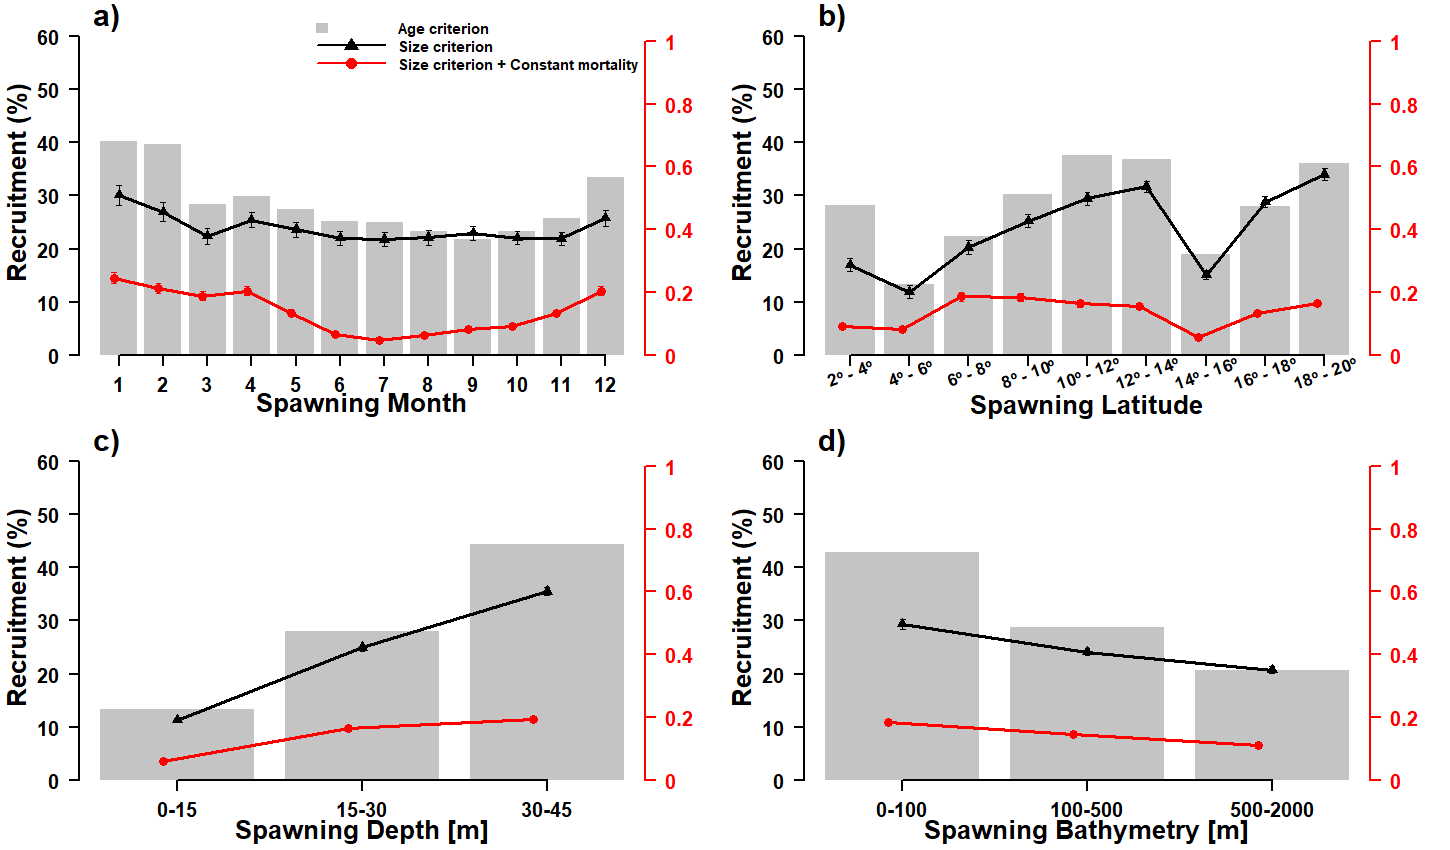
\includegraphics[width=1.0\textwidth]{figures/Chap3Case1CriterionCompar.png}
	\centering
	\caption{Percentage of recruited larvae of Peruvian anchovy obtained for different a) spawning months, b) spawning latitudes, c) spawning depths and d) isobaths delimiting spawning areas horizontally using different criteria for recruitment (size criteria -black lines-, size criteria plus constant daily mortality -red lines-) in $Sim 5$. Recruitment values based on age criteria -grey bars- were taken from $Sim 4$.}
	\label{Chap3Case1CriterionCompar}
\end{figure}

\begin{figure}[H]
	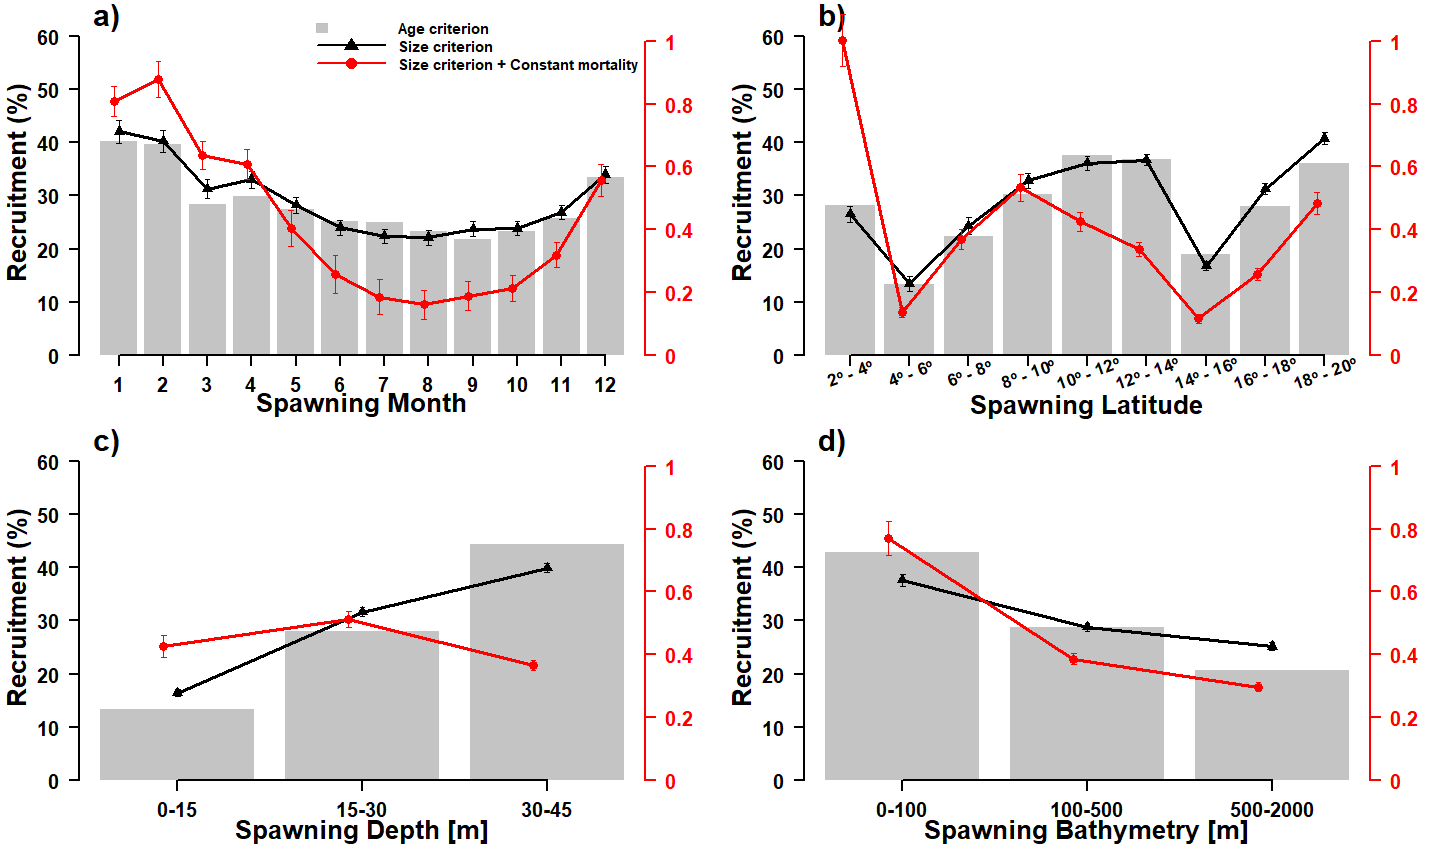
\includegraphics[width=1.0\textwidth]{figures/Chap3Case2CriterionCompar.png}
	\centering
	\caption{Same as Fig. \ref{Chap3Case1CriterionCompar} in $Sim 6$.}
	\label{Chap3Case2CriterionCompar}
\end{figure}

\begin{figure}[H]
	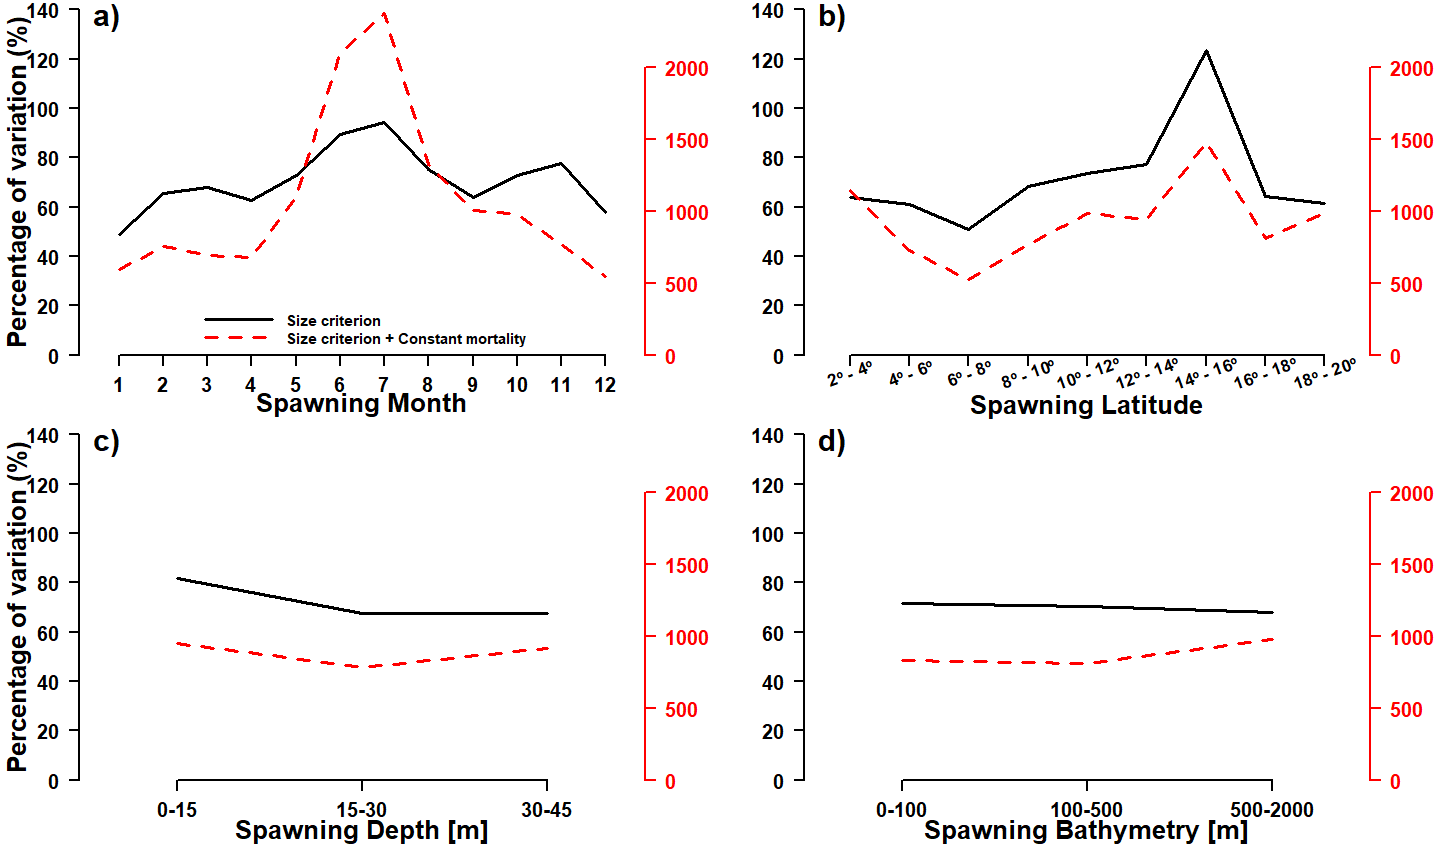
\includegraphics[width=1.0\textwidth]{figures/Chap3Case1f1.png}
	\centering
	\caption{Percentage of variation in recruitment obtained using the size criterion (black line) and the size criterion with mortality included (red dotted line) for $Sim 7$ (Case 1) relatively to $Sim 5$ (Case 1) according to a) spawning month, b) spawning latitude, c) spawning depth and d) spawning bathymetry.}
	\label{Chap3Case1f1}
\end{figure}

\begin{figure}[H]
	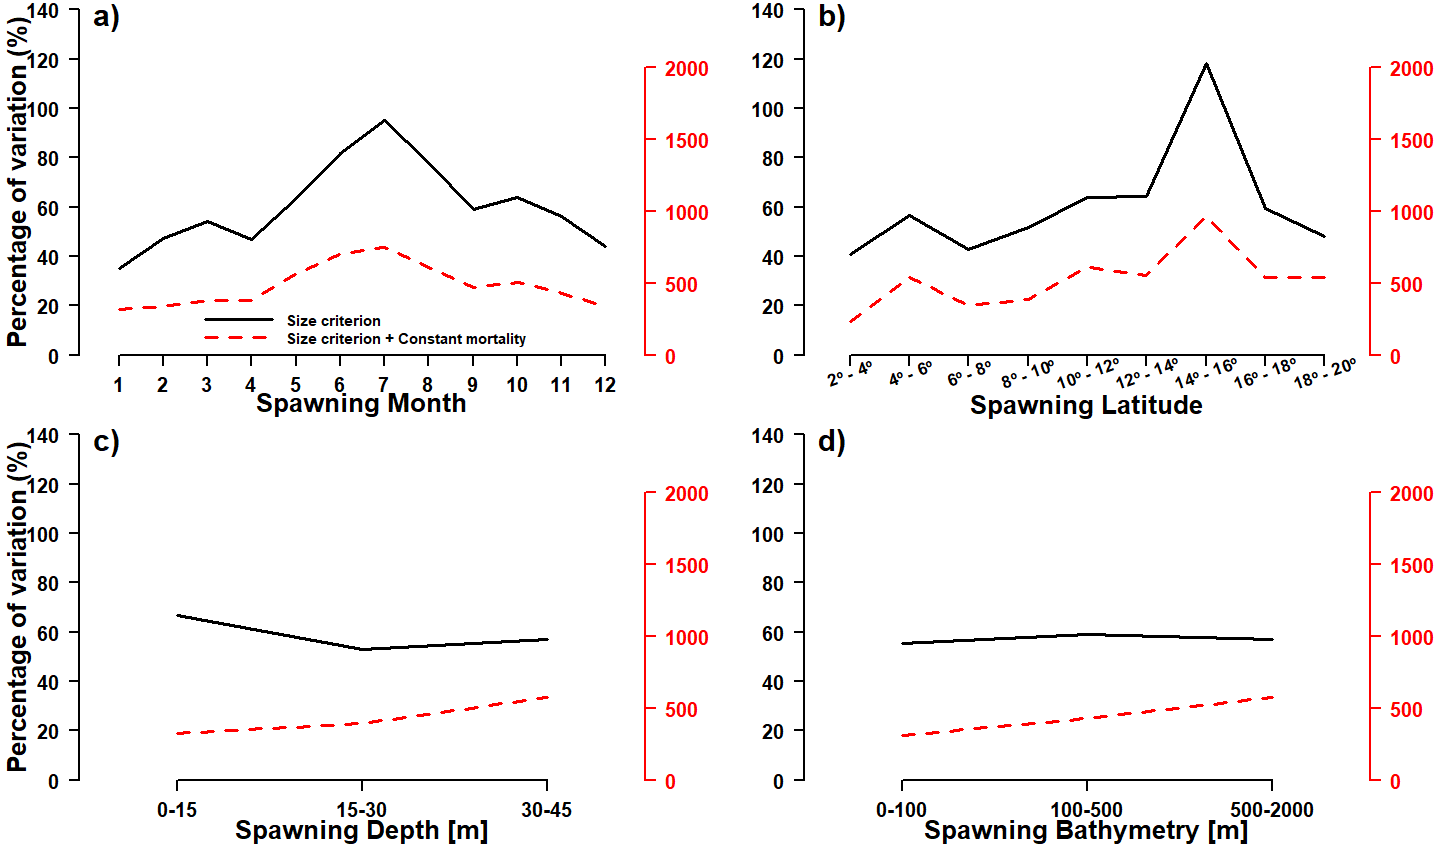
\includegraphics[width=1.0\textwidth]{figures/Chap3Case2f1.png}
	\centering
	\caption{Same as Fig \ref{Chap3Case1f1} but for $Sim 8$ (Case 2) relatively to $Sim 6$ (Case 2}
	\label{Chap3Case2f1}
\end{figure}

\begin{figure}[H]
	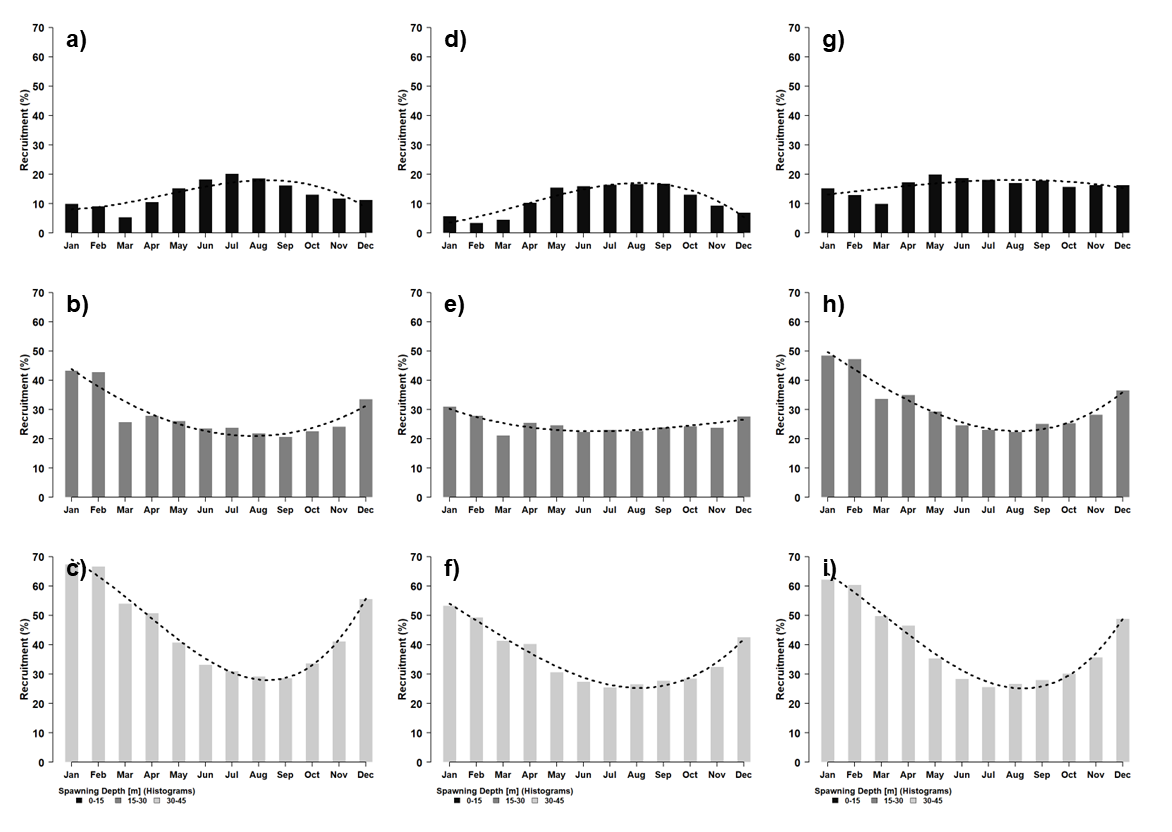
\includegraphics[width=1.0\textwidth]{figures/Chap3DepthLevels.png}
	\centering
	\caption{Percentage of recruited larvae of Peruvian anchovy obtained for different spawning depths in $Sim 4$ criterion 1 (a, b, c), $Sim 5$ criterion 2 (d, e, f) and $Sim 6$ criterion 2 (g, h, i). Spawning depth is (a, d, g) 0 - 15 $m$, (b, e, h) 15 - 30 $m$, (c, f, i) 30 - 45 $m$. The dotted curves are third degree polynomial models fitted to the recruitment patterns.}
	\label{Chap3DepthLevels}
\end{figure}

When a size criterion was used for recruitment (criterion 2), the corresponding age at which individuals recruited was very variable, ranging from 20 to 90 days (Fig. \ref{Chap3MapAgeRecruSim5Sim6}). In $Sim 5$ (Case 1), the central coastal zone of the \acrshort{nhcs} was the most favorable to early recruitment (Fig. \ref{Chap3MapAgeRecruSim5Sim6}a), while $Sim 6$ (Case 2) also favored the central coastal zone and also the northern zone showing much lower recruitment ages than $Sim 5$ (Fig. \ref{Chap3MapAgeRecruSim5Sim6}b). In Case 1, daily recruitment started at an age of $\sim$35 days for all spawning depth levels, and peaked at a similar age of $\sim$50 days (Fig. \ref{Chap3LinesAgeRecruSim5Sim6}a). Upon application of a mortality rate, as illustrated in Fig. \ref{Chap3LinesAgeRecruSim5Sim6}c, recruitment patterns become more uniform. However, a notable change is observed, in which the average depth (15-30 $m$) is slightly more favorable in terms of the age at which individuals are recruited. In Case 2, individuals in the northern part of the \acrshort{nhcs} recruited as early as $\sim$20 days and the daily recruitment peaked at ages $\sim$25, $\sim$35 and $\sim$45 days for depth levels 0 - 15, 15 - 30 and 30 - 45 $m$, respectively (Fig. \ref{Chap3LinesAgeRecruSim5Sim6}b), however, upon application of a mortality rate, it becomes evident that the shallowest zone (0 - 15 $m$) exhibits the greatest degree of favorable recruitment potential (Fig. \ref{Chap3LinesAgeRecruSim5Sim6}d).\\

\begin{figure}[H]
	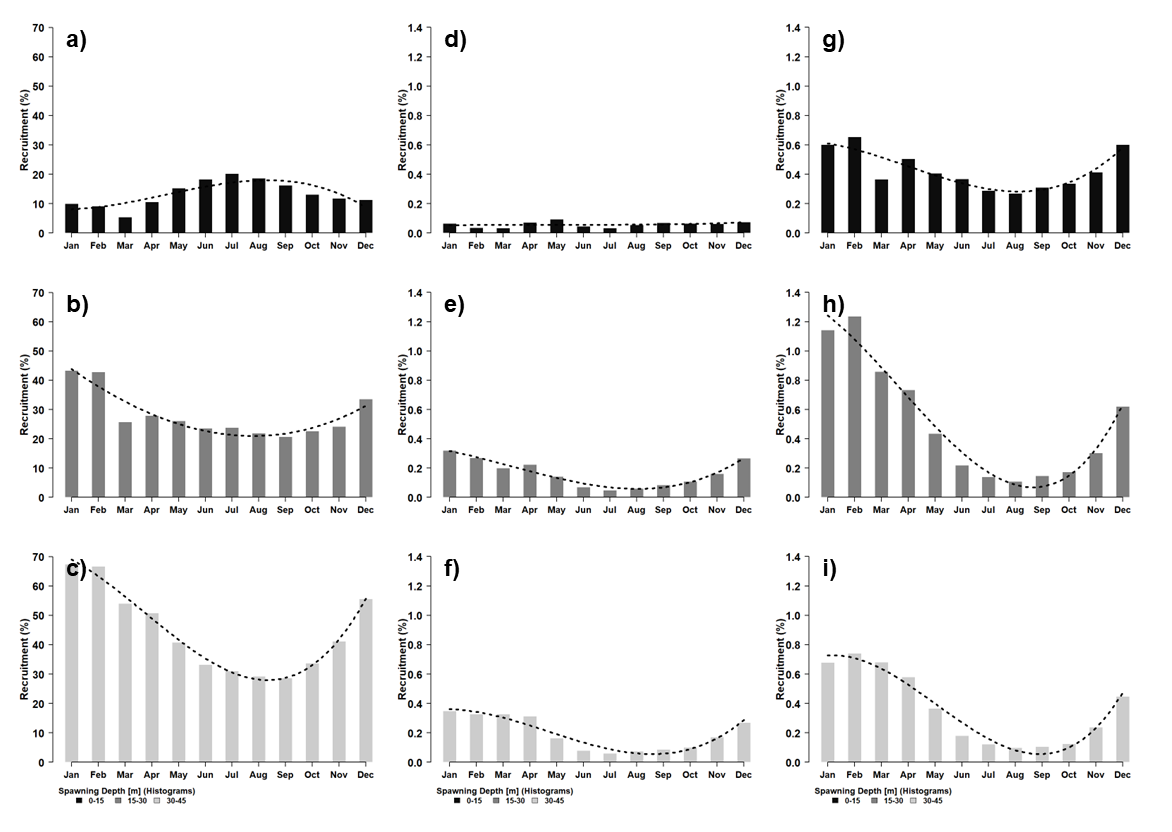
\includegraphics[width=1.0\textwidth]{figures/Chap3DepthLevelsMortality.png}
	\centering
	\caption{Same as Fig. \ref{Chap3DepthLevels} but with mortality included in $Sim 5$ and $Sim 6$ (criterion 3).}
	\label{Chap3DepthLevelsMortality}
\end{figure}

\begin{figure}[H]
	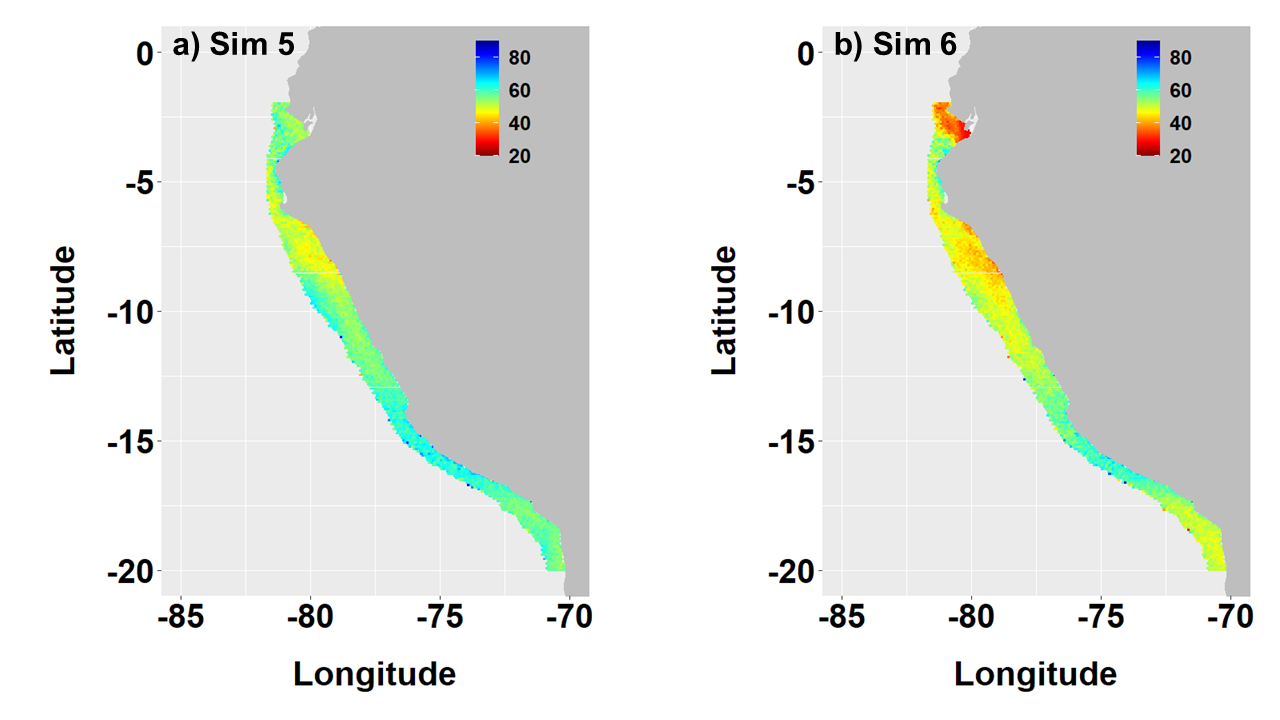
\includegraphics[width=1.0\textwidth]{figures/Chap3MapAgeRecruSim5Sim6.png}
	\centering
	\caption{Spatial distribution of average age at recruitment for a) $Sim5$ and b) $Sim6$.}
	\label{Chap3MapAgeRecruSim5Sim6}
\end{figure}

\begin{figure}[H]
	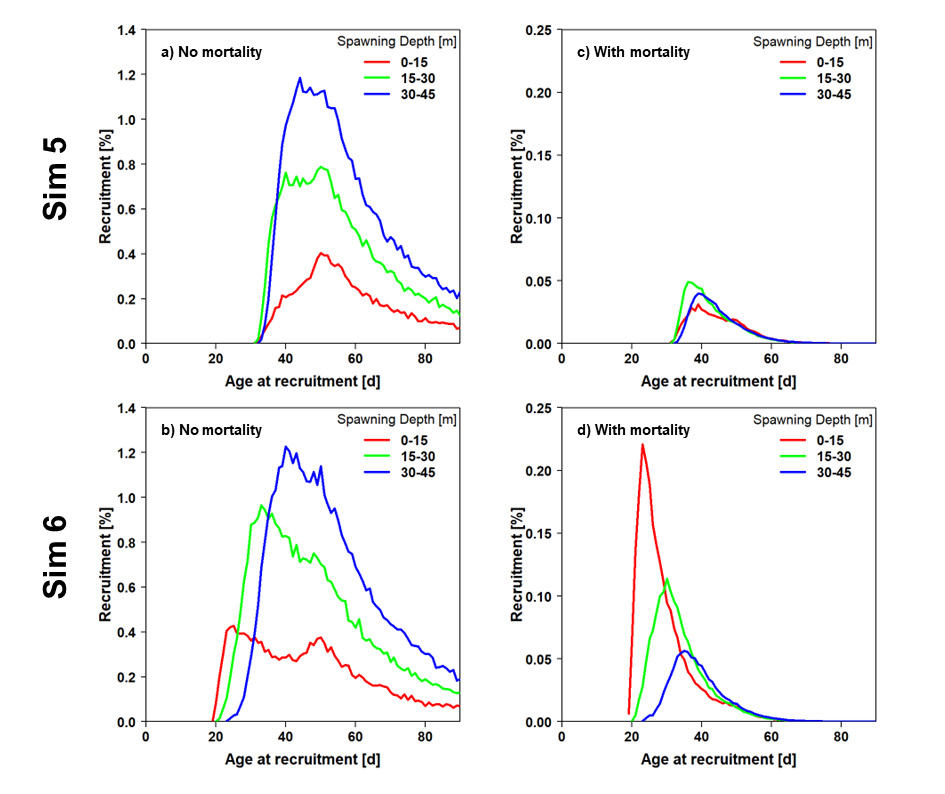
\includegraphics[width=1.0\textwidth]{figures/Chap3LinesAgeRecruSim5Sim6.png}
	\centering
	\caption{Spatial distribution of average age at recruitment for a) $Sim5$ and b) $Sim6$.}
	\label{Chap3LinesAgeRecruSim5Sim6}
\end{figure}

The amount of larvae recruiting according to their spawning location was also very variable along the coast, ranging from 0 to 150 $ind/m^2$ without mortality (Fig. \ref{Chap3DistPartiMapEgg}a, c) and from 0 to 2 $ind/m^2$ cell with mortality (Fig. \ref{Chap3DistPartiMapEgg}c, d). For Case 2 there were three spawning spots favorable to recruitment in the north, center and south of the domain (Fig. \ref{Chap3DistPartiMapEgg}c, d). For Case 1 the northern zone was no longer favorable but the central and southern zones remained (Fig. \ref{Chap3DistPartiMapEgg}a, b), which is more consistent with the spatial distribution of Peruvian anchovy egg density ($eggs/m^2$) derived from field surveys (Fig. \ref{Chap3DistPartiMapEgg}e).\\

\begin{figure}[t]
	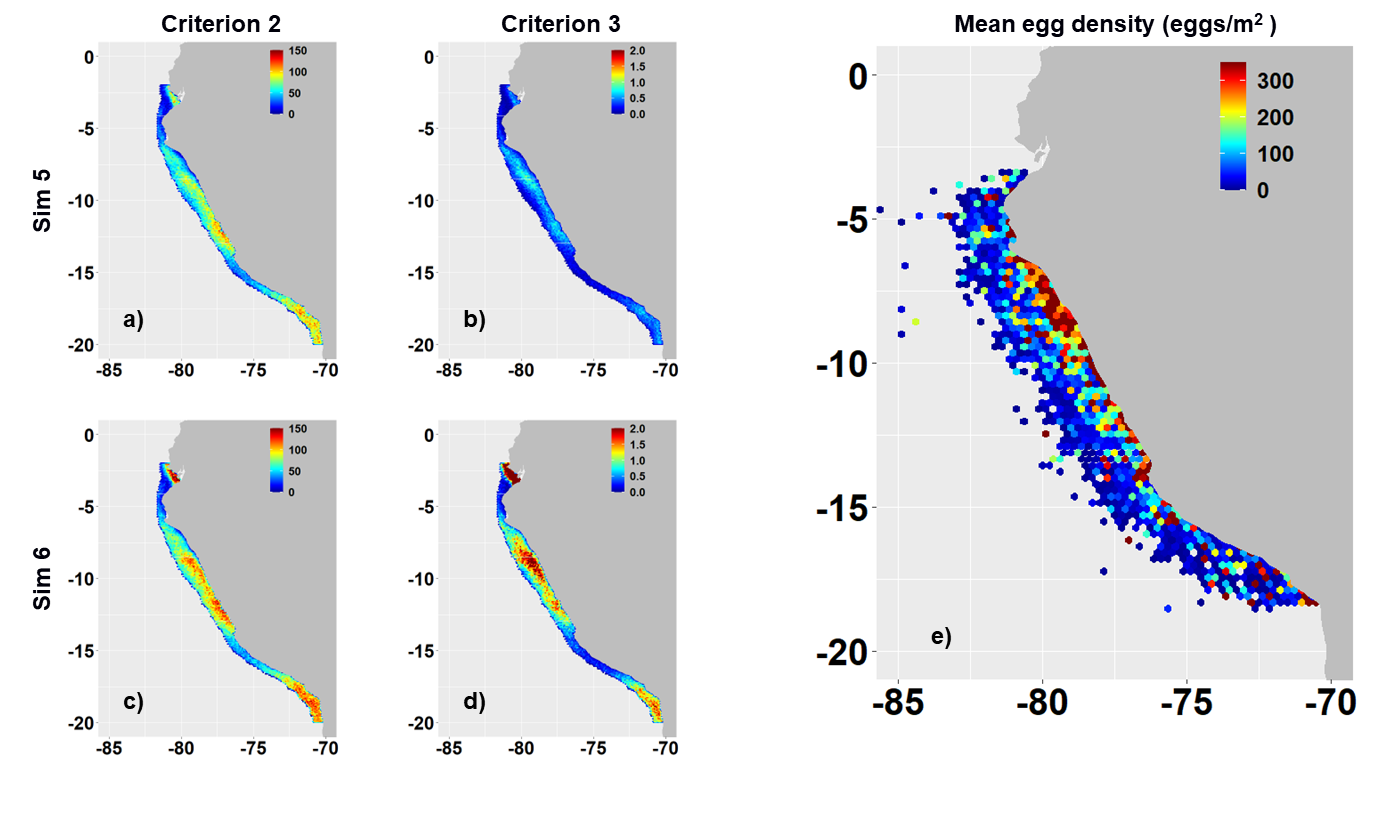
\includegraphics[width=1.0\textwidth]{figures/Chap3DistPartiMapEgg.png}
	\centering
	\caption{Spatial distribution of the average number ($ind/m^2$) of simulated Peruvian anchovy larvae recruiting according to their spawning location obtained with (a, b) $Sim 5$ and (c, d) $Sim 6$ using recruitment criterion 2 (no mortality) (a, c) and 3 (with mortality) (b, d). (e) Spatial distribution of Peruvian anchovy mean egg density ($eggs/m^2$) derived from IMARPE field surveys from year 1961 to 2016. Note that cell grid was 0.1\textdegree x 0.1\textdegree in a - d and 0.25\textdegree x 0.25\textdegree in e).}
	\label{Chap3DistPartiMapEgg}
\end{figure}

\clearpage
\section{Results of interannual simulations}\label{Chap3Resu2}

Figure \ref{Chap3TempMesoInter} illustrates the mean depth of the entire spawning zone (2 \textdegree -20 \textdegree S), as described in Figure \ref{Chap3SpawningZone}, for the forcing variables of the growth model (temperature and food). As it is an interannual forcing, it is possible to observe the effects of El Niño. During the El Niño periods (82/83 and 97/98), the temperature increased to 28 \textdegree C at the surface and to 22 \textdegree C in the deepest layer at 45 $m$. The aforementioned events represent the most extreme occurrences; however, other episodes of natural temperature increase relatives to the summer season were also observed, which did not exceed the 20 $m$ depth layer and with less intensity than extreme events (Fig. \ref{Chap3TempMesoInter}, upper panel). On the other hand, the food available in the environment was affected, decreasing its value in the same extreme events. In addition, it was observed that the layer between 0 - 20 $m$ is the one that concentrates the highest amount of food (Fig. \ref{Chap3TempMesoInter}, lower panel).\\

\begin{figure}[H]
	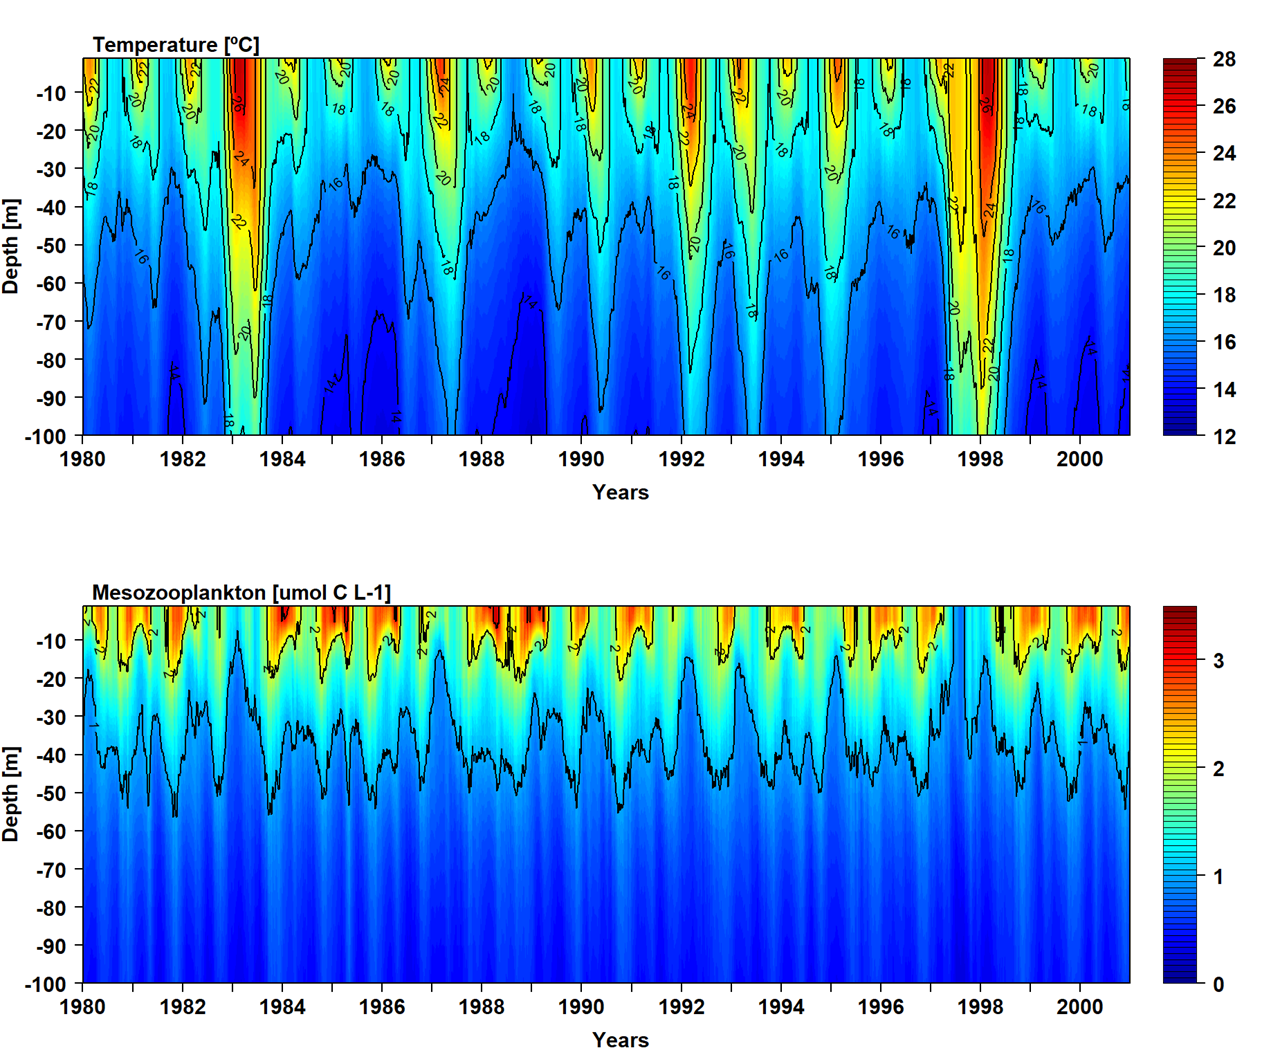
\includegraphics[width=1.0\textwidth]{figures/Chap3TempMesoInter.png}
	\centering
	\caption{Temperature (\textdegree C, upper panel) and mesozooplankton (umol, CL-1 bottom panel) vertical average from spawning zone of used as forcing for the interannual simulations of Peruvian anchovy recruitment.}
	\label{Chap3TempMesoInter}
\end{figure}

Figure \ref{Chap3CT_Depth_f_Inter} illustrates the impact of temperature and food on the growth of individuals, employing temperature correction curves (Cases 1 and 2) and a functional response for food concentration. A high value of the temperature correction implies a faster metabolism, while values close to zero are unfavorable for individuals. In Case 1, when the metabolism rate reaches a maximum at 19 \textdegree C, the negative effect during El Niño events is evident, extending to 80 meters depth (Fig. \ref{Chap3CT_Depth_f_Inter}, upper panel). Conversely, in Case 2 (when the metabolic rate reaches a maximum at 23 \textdegree C), this negative effect was concentrated in the first 45 meters depth (Fig. \ref{Chap3CT_Depth_f_Inter}, middle panel). Furthermore, Case 1 demonstrated a more frequent unfavorable effect during the study period (1980-2000) than Case 2. Finally, we observed that the value of the functional response, which limits the assimilation of individuals, remained at values of 0.5 (between 0 - 20 $m$) with the exception of extreme events where much lower values were observed, indicating a feeding deficiency (Fig. \ref{Chap3CT_Depth_f_Inter}, lower panel).\\

Fig. \ref{Chap3RecruitCase1Case2Inter} shows the difference between recruitment rates for Case 1 ($Sim 9$) and Case 2 ($Sim 10$). Both simulations show a decrease in recruitment rates during extreme events, however, Case 1 is more evident. Case 2 showed a favorable effect in the previous year to the extreme event, but then a decline in recruitment rates especially at the beginning of year 1998.\\

Analyses of variance (ANOVA) for $Sim 9$ (Case 1, Table \ref{ANOVAsim9}) and $Sim 10$ (Case 2, Table \ref{ANOVAsim10}) yielded comparable results. Spawning year accounted for 4.07 \% and 3.78 \%, respectively, while spawning month exhibited a relatively modest effect in Case 1 (0.39 \%) but a more pronounced one in Case 2 (3.55 \%). Spawning depth exhibited comparable and not dissimilar percentages of variance explanation (23.25 \% and 18.64 \%, respectively). Spawning bathymetry showed values of 4.70 \% and 7.56 \%, indicating a difference that was not as pronounced as that observed for spawning month. Finally, spawning latitude exhibited no significant difference between Case 1 and Case 2 (4.17 \% and 4.35 \%, respectively). The combinations of factors did not yield values that could be considered significant for differentiating Case 1 and Case 2 at the level of interannual simulations.\\

Given the importance of spawning depth for both simulations, it is necessary to consider the isolated effect of this factor. (Fig. \ref{Chap3RecruitCase1Case2InterDepths}) showed a high negative effect of extreme events on the three spawning depths in Case 1 ($Sim 9$, Fig. \ref{Chap3RecruitCase1Case2InterDepths}, left panels). This is less evident in Case 2 (($Sim 10$, Fig. \ref{Chap3RecruitCase1Case2InterDepths}, right panels)), where even in the shallowest depth (0-15 m), a favorability was observed before the onset of the extreme event. In the middle depth zone (15- 30 m) a negative effect of extreme events was observed, but then in the deeper zone (30 - 45 m) this effect was difficult to notice.

\begin{figure}[H]
	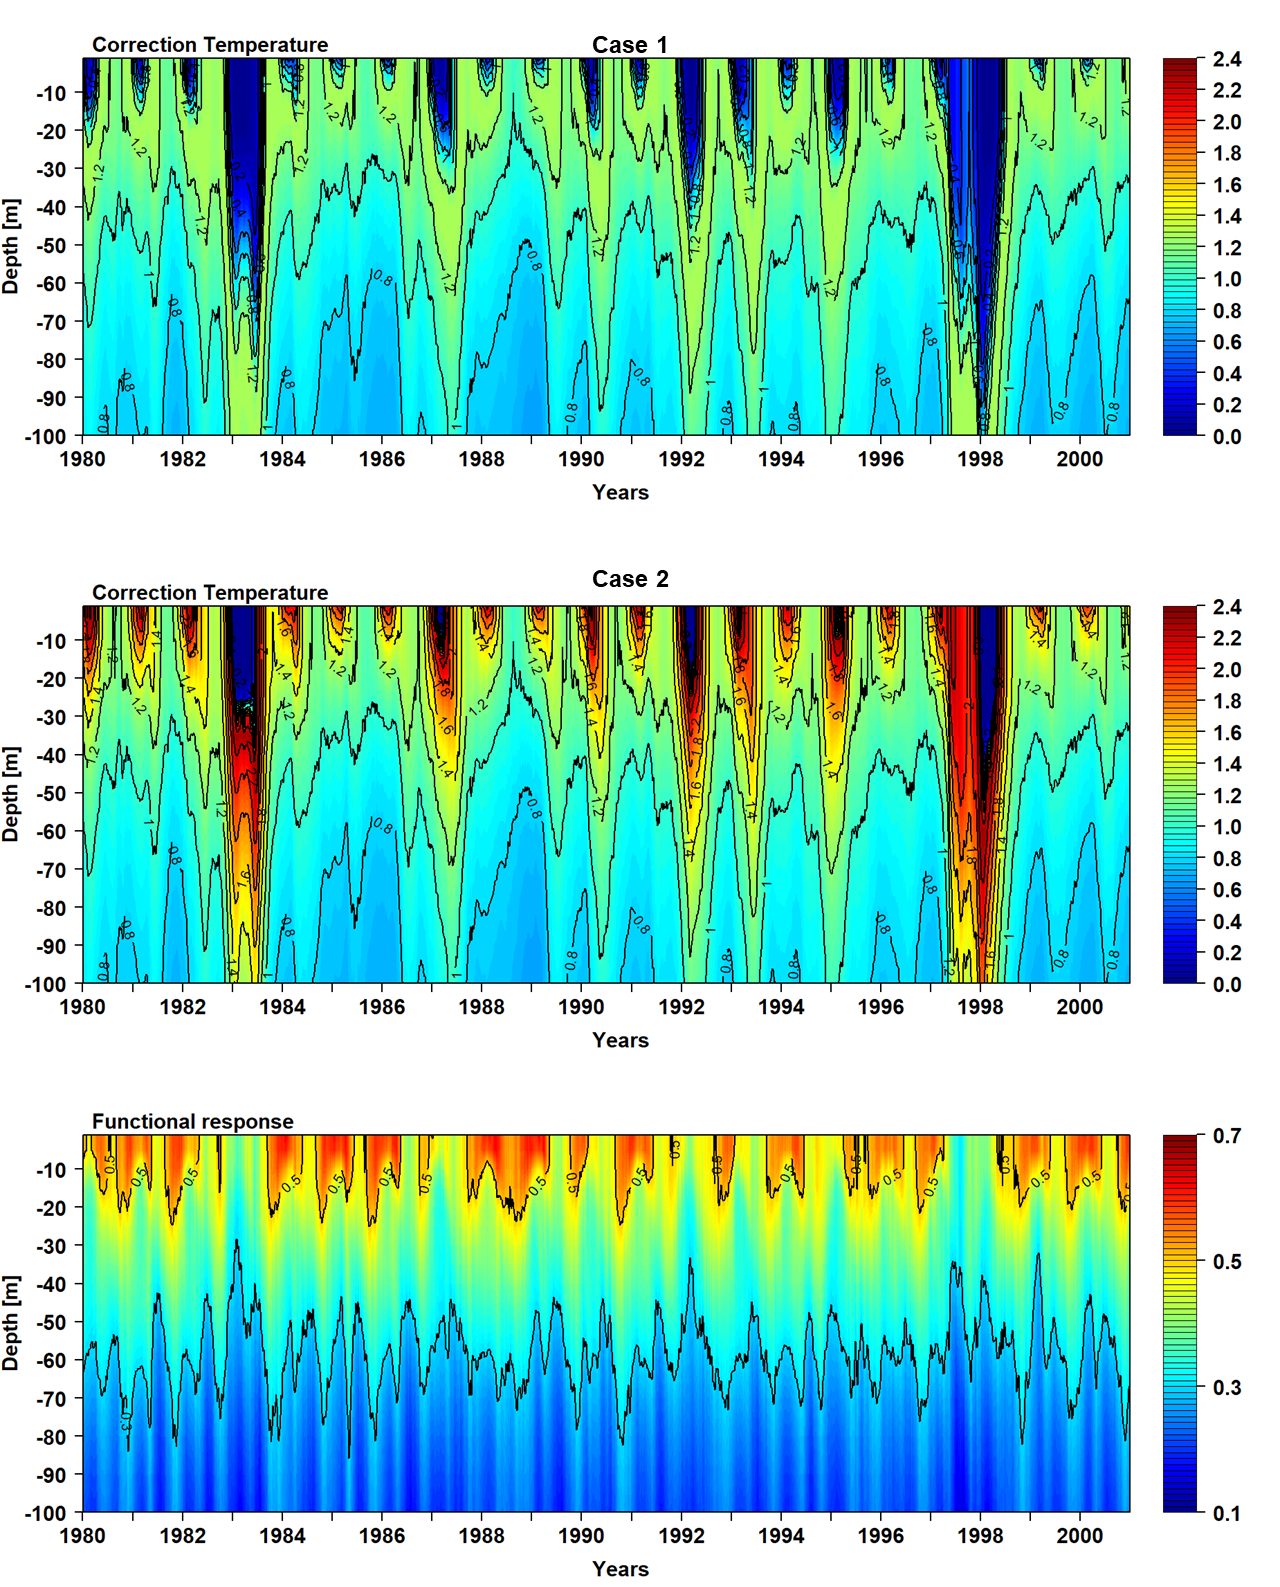
\includegraphics[width=1.0\textwidth]{figures/Chap3CT_Depth_f_Inter.png}
	\centering
	\caption{Spawning zone vertical average of temperature correction values for Case 1 (upper panel), Case 2 (middle panel) and the functional response for $K$ (half-saturation constant) fixed with a value of 1.6 (bottom panel).}
	\label{Chap3CT_Depth_f_Inter}
\end{figure}

\begin{figure}[H]
	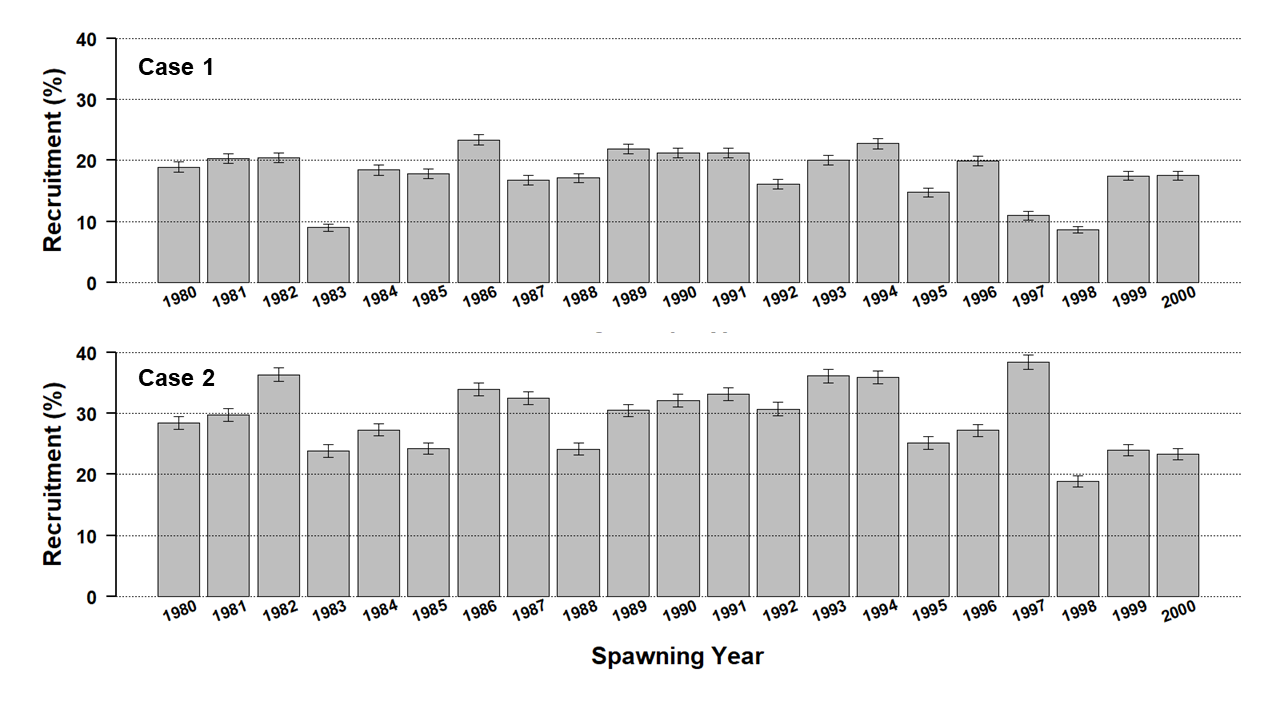
\includegraphics[width=1.0\textwidth]{figures/Chap3RecruitCase1Case2Inter.png}
	\centering
	\caption{Percentage of recruited larvae of Peruvian anchovy obtained from interannual simulation for Case 1 ($Sim 9$, upper panel) and Case 2 ($Sim 10$, bottom panel).}
	\label{Chap3RecruitCase1Case2Inter}
\end{figure}

%\begin{landscape}
\begin{table}[H]
\centering
\begin{adjustbox}{width=0.9\textwidth}
\small
\begin{tabular}{c|r|r|r|r|r|r}
\hline
                                  &
	\textbf{Df}                   &
	\textbf{Sum Sq}               &
	\textbf{Mean Sq}              &
	\textbf{F-value}    		   &
	\textbf{Pr (\textgreater{F})} &
	$\mathbf{\% Exp}$      \\
\hline
Year                  & 20	 & 845551.35  & 42277.57   & 258.49	   & 0	         & 4.07\\
Month                 & 11	 & 81363.69	  & 7396.70    & 45.22	   & 3.51E-99	 &0.39  \\
Depth                 & 2	 & 4830381.85 & 2415190.93 & 14766.83 & 0 			 & 23.25 \\
Bathymetry            & 2	 & 976098.17  & 488049.08  & 2984.00  & 0	         &4.70 \\
Latitude              & 8	 & 866683.05  & 108335.38  & 662.38	   & 0			 & 4.17\\
Year x Month          & 220 & 1011928.10 &	4599.67    & 28.12    & 0	         & 4.87  \\
Year x Depth          & 40	 & 268208.22  & 6705.21	   & 41.00	   & 3.1069e-313 & 1.29 \\
Year x Bathymetry     & 40  & 100511.81  & 2512.80	   & 15.36	   & 2.85E-103	 & 0.48 \\
Year x Latitude       & 160 & 779153.64  &	4869.71	   & 29.77	   & 0	         & 3.75  \\
Month x Depth         & 22	 & 392004.06  & 17818.37  &108.94	   & 0	         & 1.89 \\
Month x Bathymetry    & 22	 & 77401.74	  & 3518.26	   &21.51	   & 7.35E-86	 & 0.37  \\
Month x Latitude      & 88	 & 903658.26  & 10268.84  & 62.79	   & 0	         & 4.35  \\
Depth x Bathymetry    & 4	 & 64586.37	  & 16146.59   &98.72	   & 7.45E-84	 & 0.31  \\
Depth x Latitude      & 16	 & 358956.59  & 22434.79  & 137.17	   & 0	         &1.73 \\
Bathymetry x Latitude & 12	 & 794674.55  & 66222.88  & 404.90	   & 0	         & 3.83  \\
Residuals             & 51490	& 8421456.73 &163.56  & & 						 & 40.54\\
\hline
\end{tabular}
\end{adjustbox}
\caption{ANOVA of recruitment rates for $Sim 9$ (Case 1).}
\label{ANOVAsim9}
\end{table}
%\end{landscape}

%\begin{landscape}
\begin{table}[H]
\centering
\begin{adjustbox}{width=0.9\textwidth}
\small
\begin{tabular}{c|r|r|r|r|r|r}
\hline
                                  &
	\textbf{Df}                   &
	\textbf{Sum Sq}               &
	\textbf{Mean Sq}              &
	\textbf{F-value}    		   &
	\textbf{Pr (\textgreater{F})} &
	$\mathbf{\% Exp}$      \\
\hline
Year                  & 20    & 1391210.69  & 69560.53   & 265.92   & 0                   & 3.78  \\
Month                 & 11    & 1306548.20  & 118777.11  & 454.06   & 0                   & 3.55  \\
Depth                 & 2     & 6854738.93  & 3427369.47 & 13102.18 & 0                   & 18.64 \\
Bathymetry            & 2     & 2780996.10  & 1390498.05 & 5315.61  & 0                   & 7.56  \\
Latitude              & 8     & 1601243.32  & 200155.41  & 765.16   & 0                   & 4.35  \\
Year x Month          & 220   & 2136202.06  & 9710.01    & 37.12    & 0                   & 5.81  \\
Year x Depth          & 40    & 234791.26   & 5869.78    & 22.44    & 9.10E-161           & 0.64  \\
Year x Bathymetry     & 40    & 191622.73   & 4790.57    & 18.31    & 3.88E-127           & 0.52  \\
Year x Latitude       & 160   & 1626858.91  & 10167.87   & 38.87    & 0                   & 4.42  \\
Month x Depth         & 22    & 1221642.66  & 55529.21   & 212.28   & 0                   & 3.32  \\
Month x Bathymetry    & 22    & 162392.80   & 7381.49    & 28.22    & 2.11E-116           & 0.44  \\
Month x Latitude      & 88    & 1064069.64  & 12091.70   & 46.22    & 0                   & 2.89  \\
Depth x Bathymetry    & 4     & 95138.41    & 23784.60   & 90.92    & 3.64E-77            & 0.26  \\
Depth x Latitude      & 16    & 1033328.18  & 64583.01   & 246.89   & 0                   & 2.81  \\
Bathymetry x Latitude & 12    & 1610910.69  & 134242.56  & 513.18   & 0                   & 4.38  \\
Residuals             & 51487 & 13468365.16 & 261.59     &          &                     & 36.62 \\
\hline
\end{tabular}
\end{adjustbox}
\caption{ANOVA of recruitment rates for $Sim 10$ (Case 2).}
\label{ANOVAsim10}
\end{table}
%\end{landscape}

\begin{figure}[ht]
	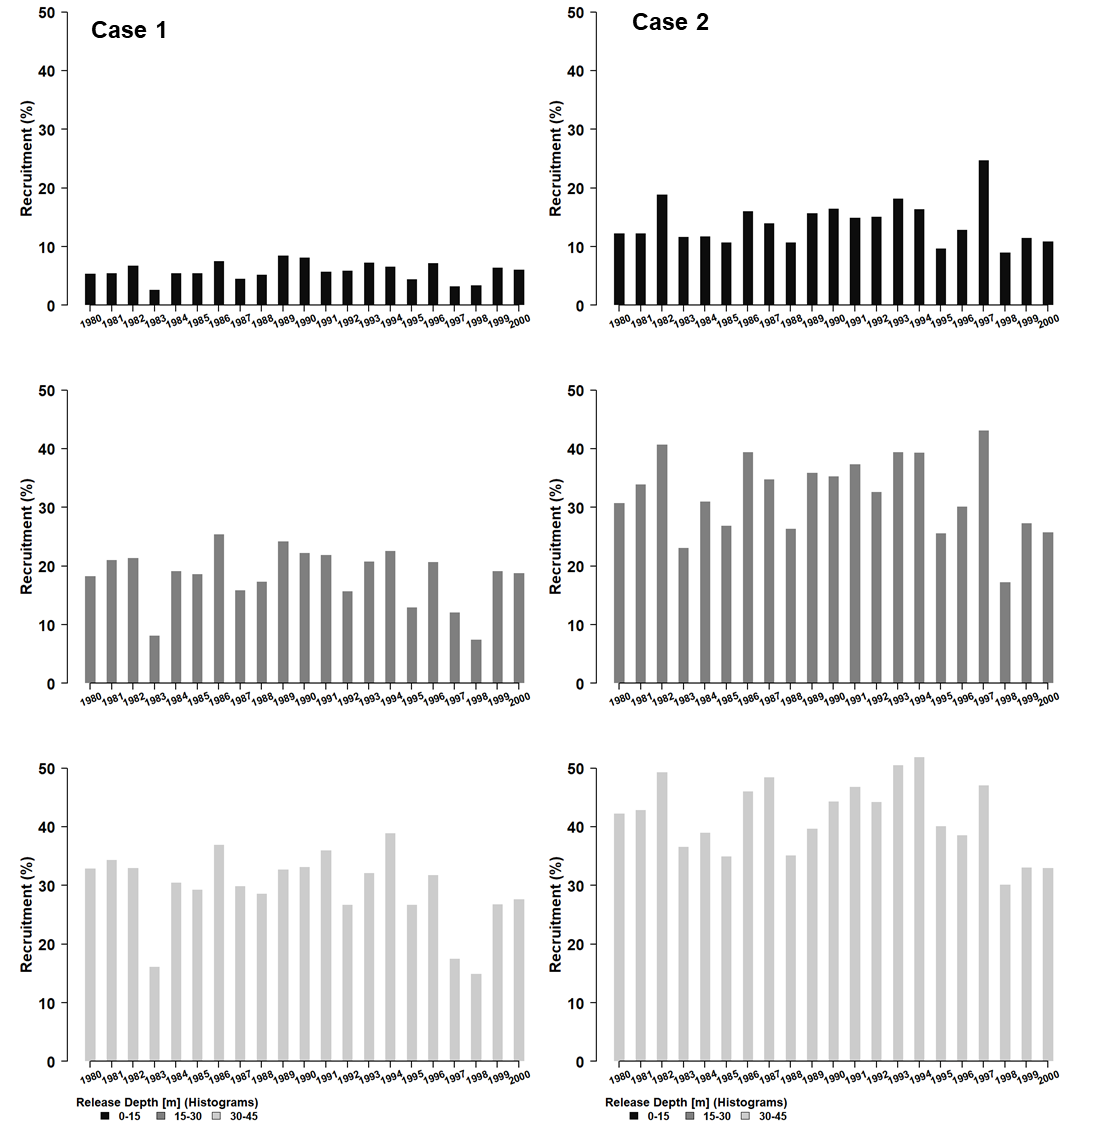
\includegraphics[width=1.0\textwidth]{figures/Chap3RecruitCase1Case2InterDepths.png}
	\centering
	\caption{Percentage of recruited larvae of Peruvian anchovy obtained from different spawning depths on the interannual simulation for Case 1 (left panels) and Case 2 (right panel).}
	\label{Chap3RecruitCase1Case2InterDepths}
\end{figure}

\clearpage
\section{Discussion of climatological simulations}\label{Chap3Disc1}

We studied larval retention and growth of the Peruvian anchovy (\textit{\gls{ringens}}) in the \acrshort{nhcs} using a biophysical model. This model was first forced by currents from a more modern configuration of a hydrodynamic model used previously at the same horizontal resolution (10 km; \cite{BrocLett2008}). We were able to replicate the general modeled patterns of larval retention obtained previously. Indeed, our results were consistent with another study aiming at answering the same scientific question but using a different dataset, thus proving the replicability of these results \citep{NAP25303}. This emphasis the robustness of the results despite the stochastic variability inherent to hydrodynamic model configurations. It was also crucial to replicate previous results before assessing the effects of new forcing products and other model components in order to avoid generating false conclusions \citep{Bake2016}. Here, in particular, we found the same opposite seasonal pattern relative to spawning depth (Fig. \ref{Chap3BrocVSFloreBarplots}) as \cite{BrocLett2008}. However, we obtained slightly higher coastal retention values during summer months for the three spawning depths considered. This result could be due to a greater stratification of the water column and to a higher spatial resolution of the wind stress forcing (weaker at the coast) in the new hydrodynamic simulations compared to the old one. Retention within the most coastal spawning zone (bathymetry 0 -100 $m$) was up to 20 \% higher in summer than in \cite{BrocLett2008}.\\

After including larval growth into our model based on the DEB theory, we explored simulations using a size criterion for retention (Fig. \ref{Chap3Case1CriterionCompar} and Fig. \ref{Chap3Case2CriterionCompar}), as opposed to an age criterion as before. Using a size criterion for retention means considering the impact of environmental variability on the planktonic life duration (PLD), which is crucial in biophysical modelling studies \citep{LettAyat2010}. Indeed, a shorter PLD, resulting from faster growth, is expected to increase local retention and therefore recruitment. Larvae that grow quicker may also escape predators, swim more efficiently and have therefore a better chance to survive \citep{Houd2008}, which was also explored in our results including mortality. In our simulations, larvae experienced temperatures ranging from $\sim$17\textdegree C in winter to $\sim$23\textdegree C in summer. The effect of temperature on growth depended on the hypothesis we made on the $C_T$ function (Eqn. \ref{C_T}) as we considered two temperature correction curves. Under the hypothesis of a max $C_T$ at $\sim$23.4\textdegree C (Case 1), the PLD could be as low as 20 days and the largest recruitment was found in summer in the Guayaquil Bay. However, this bay lies at the northern limit of \textit{\gls{ringens}} distribution \citep{CaldAyor2020}, and large recruitment of Peruvian anchovy has not been observed there to our knowledge. Tuning model parameters in order to fit a known distribution is a way to study the ecological niche limits. For our model prediction to fit the spatial extent of the observed spawning area (thus excluding the Guayaquil Bay, Fig. \ref{Chap3DistPartiMapEgg}e), we had to change the $C_T$ function such that its maximum value occurs at $\sim$19\textdegree C. In this case the average \acrshort{pld} of simulated recruited larvae was $\sim$50 days, which is in the order of in situ and laboratory observations \citep{PaloMuck1987}. Furthermore, \citep{CastPena2022} showed that the main habitat temperature range of adult anchovy population was 16-24\textdegree C, which is consistent with an optimal larval growth temperature around the middle of this range. However, the hypothesis that temperature would be the main factor limiting larval growth for individuals in the Guayaquil Bay should be challenged by new laboratory experiments designed to identify the upper temperature limit for larval growth. Indeed, current experiments found the fastest growth at 19\textdegree C for larval stages but did not investigate higher temperature values \citep{RiouOfel2021}. Some preliminary results tend to indicate for juvenile stages reduction of ingestion rate from 21\textdegree C (unpublished data), which would impact the growth rate. So, more laboratory experiments should be designed specifically to identify the shape of the $C_T$ function for \textit{\gls{ringens}}. Our results obtained with a 19\textdegree C maximum $C_T$ (Case 1) are also in line with \cite{XuChai2013} who found a rather adverse effect of inter-annual variability, specifically during the El Niño period, where the number of days to reach recruitment increased and survival decreased considerably.\\

In simulations where food was considered as not limiting larval growth, we found similar results as in simulations where both food and temperature were limiting. This result contrasts with \cite{ThomDuma2016} who used a similar bio-energetic approach as ours to study oyster larvae growth and recruitment in Polynesia. In a context where temperature variability was much smaller ($\sim$28-29\textdegree C) they found that food limitation explained most of recruitment variability. In our case, larval food limitation did not impact the seasonal pattern but it had a small impact on the spatial pattern, suggesting an average higher food limitation south of the Pisco upwelling cell ($\sim$14 – 15 \textdegree S), which is in line with a lower upwelling productivity \citep{EspiEche2017}.\\

The confirmation by laboratory experiments of a ``smooth” temperature correction function (as in Case 1 of the present simulations) for \textit{\gls{ringens}} would be consistent with the widely accepted idea that temperature is a limiting factor for anchovy blooming \citep{ChavBert2008}. However, a steeper temperature correction (Case 2) function would challenge this idea. In this latter case, other factors responsible for the northern limit of \textit{\gls{ringens}} habitat, possibly correlated with temperature, should be identified, as water masses \citep{BertSegu2004,SwarBert2008}, oxygen \citep{BertChai2011}, or food quality \citep{AyonSwar2008,CaldAyor2020} as food abundance was not found as a key limiting factor in our study. The change in species dominance shown in sediment records, corresponding to periods of environmental changes \citep{SalvField2018,SalvGuti2019}, would then be more associated to changes in stratification and circulation leading to a decrease in oxygen availability and/or decrease in ichthyoplankton retention \citep{BrocEche2013,EspiEche2021}, affecting larval vertical distribution.\\

In Peru, small pelagic fish monitoring is based on spawning biomass estimation and egg and larvae surveys \citep{PaulSori1987,Ayon2000,GutiCast2012} without explicitly accounting for spatial features (e.g. cross-shore and vertical). However, our results shows that spatial and vertical distribution also largely impact the success of recruitment. We suggest this information should be included in coupled model and observation operational system, which allows to forecast the seasonal success of recruitment. Thus, spatial monitoring of ichthyoplankton distribution should include assessment of vertical distribution. This can be achieved using multinet or, for a faster processing of the information, in situ imaging system that may allow a rapid processing \citep{OrenRate2020}.

\clearpage
\section{Discussion of interannual simulations}\label{Chap3Disc2}

The biogeochemical model represented well the most important features relatives to increase of temperature as showed by \citep{ColaCape2008} and decrease of anchovy prey \citep{AyonSwar2011} during the extreme El Nino events. The combination of high temperatures and little food during the extreme events generated a considerable decrease in recruitment rates in Case 1. This was not as evident in Case 2, in which, because the optimum temperature threshold is higher than in Case 1, recruitment was favored at the beginning of the temperature increase period, but then a negative effect followed due to the long duration of the temperature increase.\\

The results of Case 1 interannual recruitment rates coincide with those found by \cite{XuChai2013} with a considerable decrease of recruitment during El Nino events although they used a size recruitment criterion higher than the 2 cm, as was used in the present study. This was not as evident for Case 2.\\

It should also be noted that spawning depth had a greater effect in Case 1, affecting recruitment rates during El Nino events at all 3 depths. This characteristic was not very pronounced in Case 2, suggesting that Case 1 better represented the thermal limit of the Peruvian anchovy, however, this hypothesis has yet to be demonstrated by laboratory experiments.\\

The presence of prolonged periods of unfavorable conditions for the species during El Nino events also raises a migration behavior hypothesis of the Peruvian anchovy during its juvenile/adult phase, something that could be evaluated with another modelling tool \citep{BrocAuge2018} which includes a full life cycle model and swimming ability and was successfully applied in the ecosystem of the west coast of Africa. Another possible explanation would be the deeper vertical migration of the species, but due to the long duration of El Niño events, this would only allow it to escape unfavorable conditions for a short time, having to look for more favorable areas afterwards.\\

It should also be noted that in all experiments were assumed to have a uniform spawning, something that in reality depends on the variability of the spawning biomass \citep{CahuCubi2009} and should be taken into account for further studies.

\clearpage
